\documentclass{article}
\usepackage{amsmath}
\usepackage{amsthm}
\usepackage{amsfonts}
\usepackage{amssymb}
\usepackage{bbold}
\usepackage{dsfont}
\usepackage{graphicx}
\usepackage{cleveref}
\usepackage{bm}
\usepackage{booktabs}
\usepackage{siunitx}
\usepackage{xcolor}
\usepackage[utf8]{inputenc}
\usepackage[english]{babel}
\newtheorem{definition}{Definition}
\newtheorem{example}{Example}
\newcommand{\exP}[1]{\mathrm{e}^{#1}}
\newcommand{\dif}{\mathrm{d}}
\renewcommand{\vec}[1]{\mathbf{#1}}
\newcommand{\pdagger}{{\phantom{\dagger}}}
\newcommand{\state}[1]{\vert #1\rangle}
\newcommand{\cstate}[1]{\langle #1\vert}
\newcommand{\tr}[1]{\mathrm{tr}\left\{#1\right\}}
\newcommand{\trs}[2]{\, \mathrm{tr}_{#1}\{#2\}}
\newcommand{\expc}[3]{\langle #1\vert #2 \vert #3\rangle}
\usepackage[doi=false,url=false,isbn=false,backend=bibtex,style=nature,natbib=true,sorting=none]{biblatex}
\bibliography{bib.bib}
\usepackage{geometry}
\geometry{
	a4paper,
	total={170mm,257mm},
	left=20mm,
	top=20mm,
}
\begin{document}
\title{Additional results and analyses: Transport through Peierls model}
\author{Rudolf Smorka}
\maketitle
%\tableofcontents
\section{Aim}\label{sec:Aim}
The aim is to understand the relaxation of the current through a two-site Peierls model 
\begin{equation}
	H_\mathrm{Peierls} = \varepsilon_0 (c_1^\dagger c_1^\pdagger + c_2^\dagger c_2^\pdagger)+ \omega_0 a^\dagger a -(t_0 + t_1(a^\dagger + a))(c_1^\dagger c_2^\pdagger + \mathrm{h.c.}),
\end{equation}
coupled to two leads, solved within the Ehrenfest-HEOM approach. Following Franssons work, the parameters are
\begin{align*}
	\varepsilon_0 &= -\SI{240}{\milli\electronvolt}\\
	\omega_0 &= \SI{2}{\milli\electronvolt}\\
	t_0 &= \SI{40}{\milli\electronvolt}\\
	t_1 &= \SI{4}{\milli\electronvolt}\\
	\Gamma &= \SI{10}{\milli\electronvolt}\\
	V 	&= \SI{480}{\milli\volt}\\
	T &= \SI{25}{\milli\electronvolt}.
\end{align*}
Using the creation and annihilation operators
\begin{equation}
	a^\dagger = \sqrt{\frac{m\omega_0}{2}} \left(x - \frac{i}{m\omega}p\right)
\end{equation}
the Hamiltonian is written as 
\begin{equation}
	H_\mathrm{Peierls} = \varepsilon_0 (c_1^\dagger c_1^\pdagger + c_2^\dagger c_2^\pdagger)+ \frac{m\omega_0^2 x^2}{2} + \frac{p^2}{2 m} -\left(t_0 + t_1\sqrt{2m\omega_0}x\right)(c_1^\dagger c_2^\pdagger + \mathrm{h.c.})
\end{equation}
in terms of vibrational coordinate $x$ and momentum $p$. Introducing the mass-scaled coordinate $X = \sqrt{m}x$ and momentum $P = \frac{p}{\sqrt{m}}$ yields the Hamiltonian as used in the following
\begin{equation}
	H_\mathrm{Peierls} = \varepsilon_0 (c_1^\dagger c_1^\pdagger + c_2^\dagger c_2^\pdagger)+ \frac{\omega_0^2 X^2}{2} + \frac{P^2}{2} -\left(t_0 + t_1\sqrt{2\omega_0}X\right)(c_1^\dagger c_2^\pdagger + \mathrm{h.c.}).
\end{equation}
The classical equation of motion are then
\begin{align}
	\dot{X} &= \frac{\partial \langle H\rangle}{\partial P} = P \\
	\dot{P} &= -\frac{\partial\langle  H\rangle}{\partial X} = -\omega_0^2 X +t_1\sqrt{2 \omega_0}\tr{\rho(c_1^\dagger c_2^\pdagger + \mathrm{h.c.})}.
\end{align}
This results in a strongly oscillating current for some voltages, and a non-oscillating current in other, as shown in \cref{fig:I_t_L2_F_params}. The vibrational energy with time, shown in \cref{fig:Eph_t_L2_F_params}, indicates that molecular vibrations play an important role for some voltages. Even when sampling the initial position and momentum from the thermal Wigner distribution
\begin{equation}
	\rho(X,P) = \frac{\alpha}{\pi}\exp\left[-\frac{2\alpha}{\omega}\left(\frac{P^2}{2}+\frac{\omega^2X^2}{2}\right)\right]
\end{equation} 
with $\alpha=\tanh\left(\frac{\beta\omega}{2}\right)$, and averaging the observables over the trajectories corresponding to the sampled initial conditions, 
\begin{equation}
	\langle A(t)\rangle = \frac{1}{N}\sum_j^N A(t)\big\vert_{X_0^{(j)},P_0^{(j)}},
\end{equation}
these oscillations persist (see \cref{fig:I_t_L2_F_params_avg}, \cref{fig:Eph_t_L2_F_params_avg}).
\begin{figure}[!h]
	\centering
	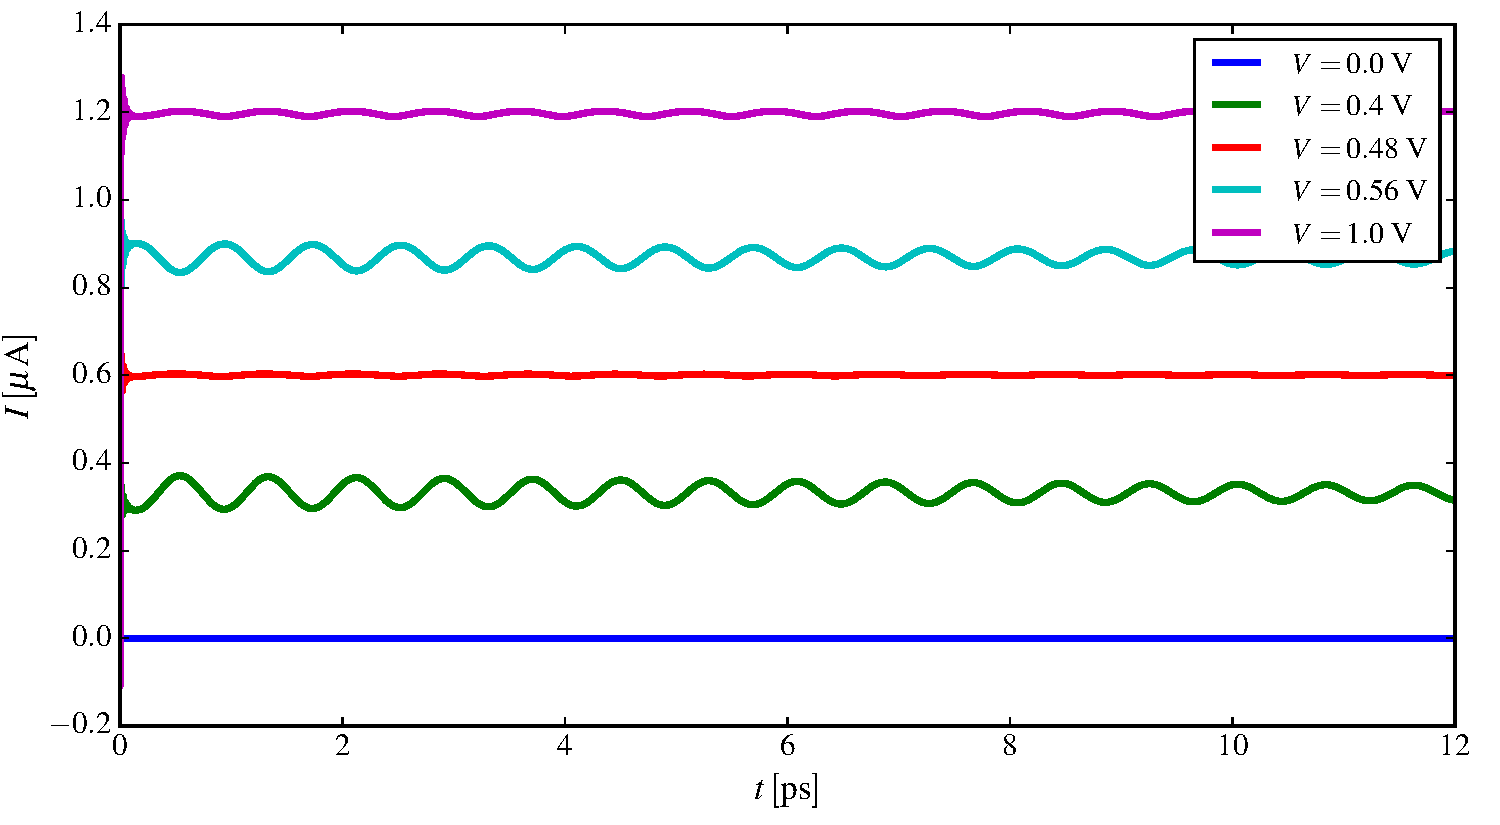
\includegraphics[width=0.9\textwidth]{figs/Peierls_L2_FranssonParams_Vvar_currents.pdf}
	\caption{Dynamics of symmetrized current for various voltage with parameters used by Fransson.}\label{fig:I_t_L2_F_params}
\end{figure}
\begin{figure}[!h]
	\centering
	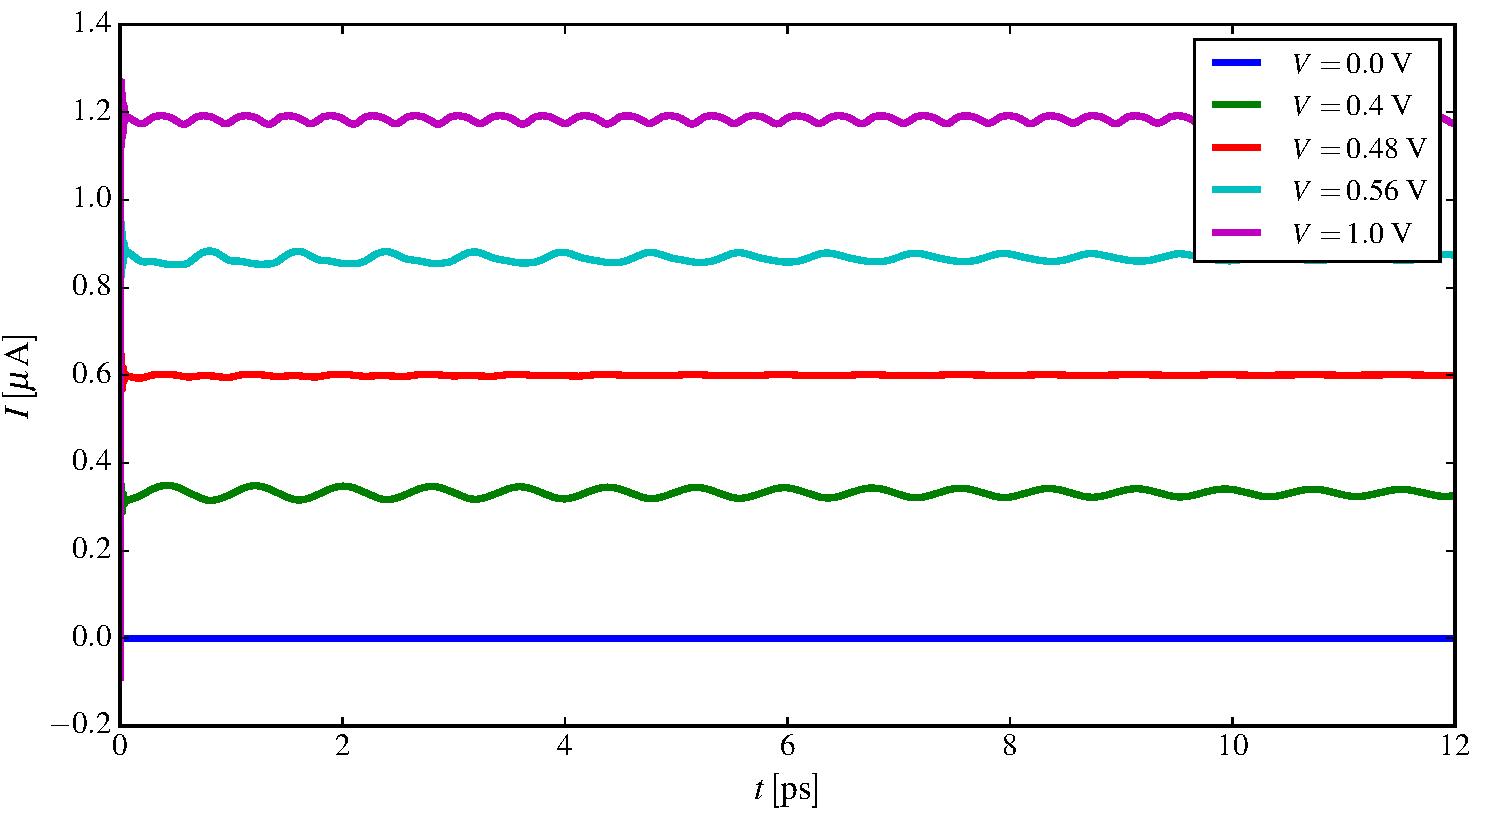
\includegraphics[width=0.9\textwidth]{figs/Peierls_L2_FranssonParams_Vvar_avg_currents.pdf}
	\caption{Same as in \cref{fig:I_t_L2_F_params}, but averaged over 6000 trajectories.}\label{fig:I_t_L2_F_params_avg}	
\end{figure}
\begin{figure}[!h]
	\centering
	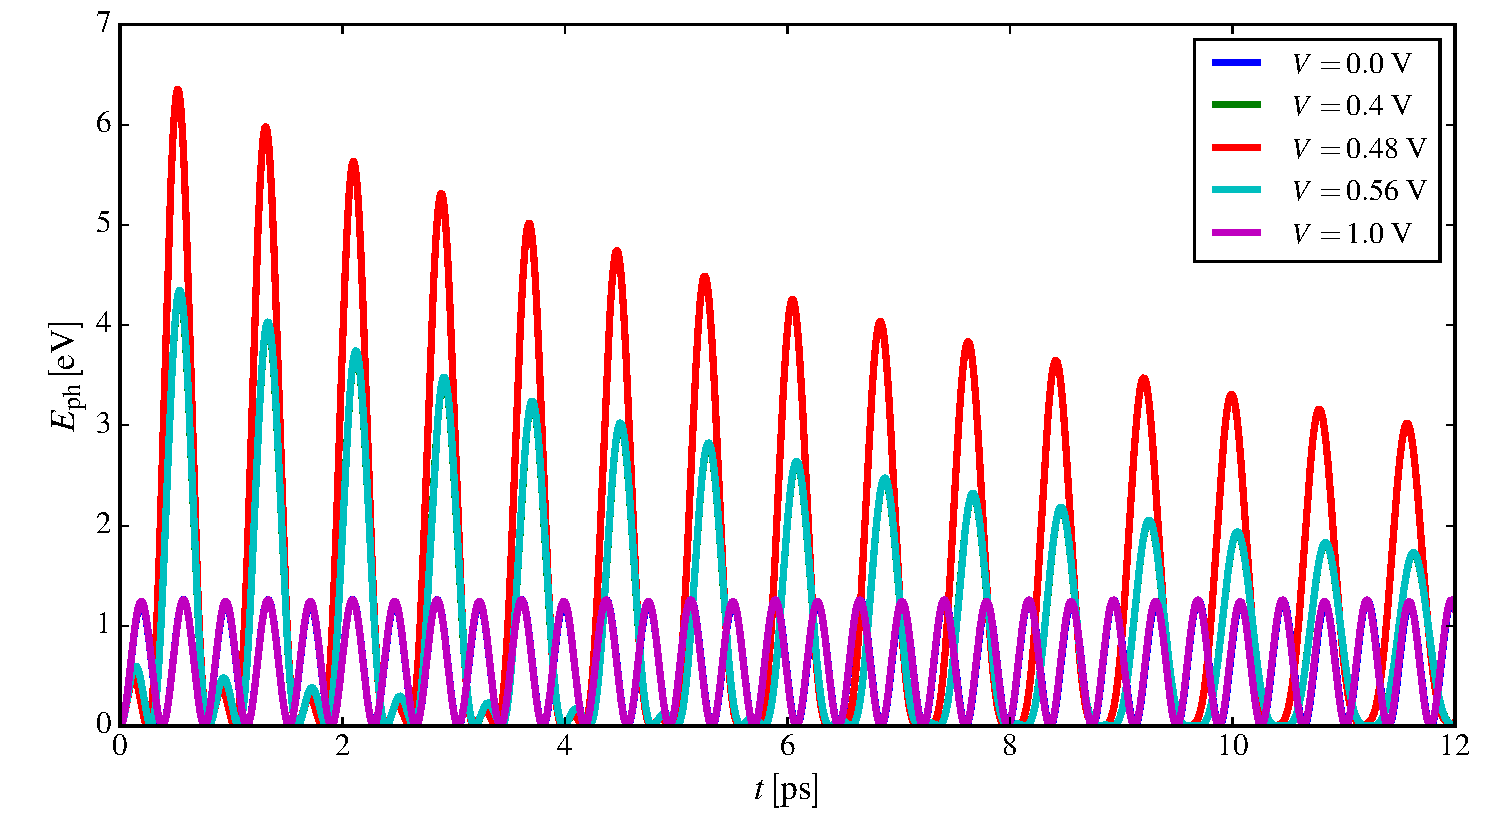
\includegraphics[width=0.9\textwidth]{figs/Peierls_L2_FranssonParams_Vvar_phonons.pdf}
	\caption{Dynamics of vibrational energy $E_\mathrm{ph} = \frac{1}{2}(\omega^2 X^2 + P^2)$ for the parameters above.}\label{fig:Eph_t_L2_F_params}
\end{figure}
\begin{figure}[!h]
	\centering
	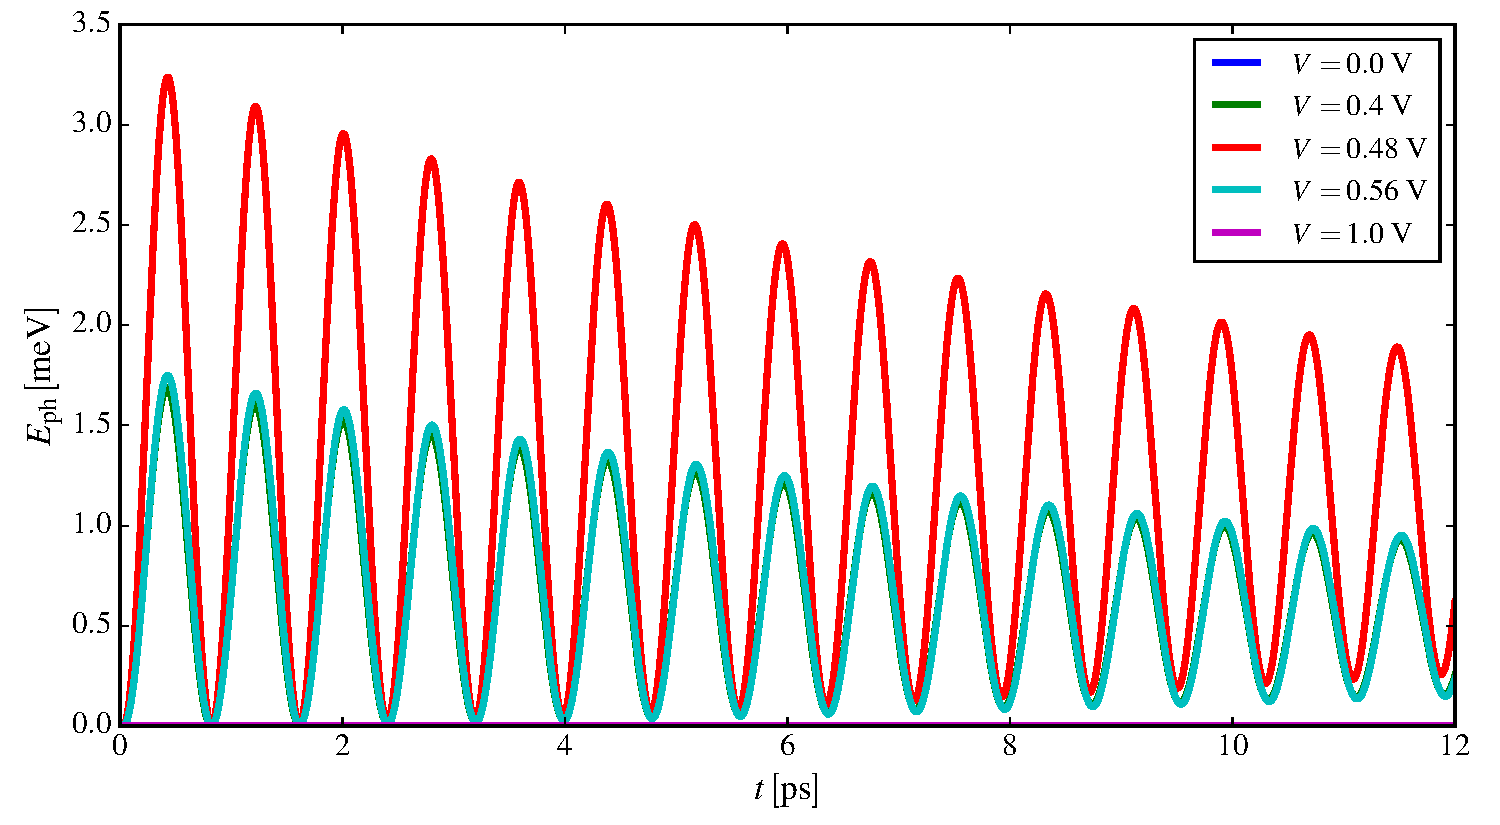
\includegraphics[width=0.9\textwidth]{figs/Peierls_L2_FranssonParams_Vvar_avg_phonons.pdf}
	\caption{Same as in \cref{fig:Eph_t_L2_F_params}, but averaged over 6000 trajectories.}\label{fig:Eph_t_L2_F_params_avg}
\end{figure}
\clearpage
\section{Analysis of the problem (I)}
The bare molecular spectrum and eigenstates are
\begin{align}
	\varepsilon_\pm &= \varepsilon_0 \pm \vert t_0 +t_1\sqrt{2\omega_0}X\vert\\
	\vert \psi_\pm\rangle &= \frac{1}{\sqrt{2}}\begin{pmatrix}
		1\\
		\pm 1
	\end{pmatrix}.
\end{align}
As the eigenenergies depend on $X$, they are time-dependent since $X$ is time-dependent in the Ehrenfest-approach.
Since the eigenstates are identical to the ones in the two-site tight binding model ($t_1 = 0$), the electron-phonon part of the Peierls Hamiltonian is diagonal in this basis 
\begin{equation}
	\tilde{H}_\mathrm{el-ph} = \begin{pmatrix}
		\langle \psi_- \vert H_\mathrm{el-ph}\vert \psi_-\rangle & \langle \psi_- \vert H_\mathrm{el-ph}\vert \psi_+\rangle\\
		\langle \psi_+ \vert H_\mathrm{el-ph}\vert \psi_-\rangle & \langle \psi_+ \vert H_\mathrm{el-ph}\vert \psi_+\rangle
	\end{pmatrix}
	= \begin{pmatrix}
		\sqrt{2\omega}t_1 X & 0\\
		0 & -\sqrt{2\omega}t_1 X
	\end{pmatrix}
\end{equation}
This means, that the electron-vibrational coupling cannot produce any coherence between eigenstates $\vert \psi_+\rangle$ and $\vert \psi_-\rangle$. Any coherence between eigenstates has to come from the coupling to the leads. The couplings in the energy-eigenbasis are
\begin{align}
	\tilde{\Gamma}_L &=  \frac{\Gamma_L}{2}\begin{pmatrix}
		1 & -1 \\
		-1 & 1
	\end{pmatrix}\\
	\tilde{\Gamma}_R &=  \frac{\Gamma_R}{2}\begin{pmatrix}
		1 & 1 \\
		1 & 1
	\end{pmatrix}\\
\end{align}
where $\Gamma_L, \Gamma_R$ are constant coupling of the problem in the site-basis. A schematic of the transformed system is shown in \cref{fig:Schematic_Peierls_transformed}.
\begin{figure}[!h]
	\centering
	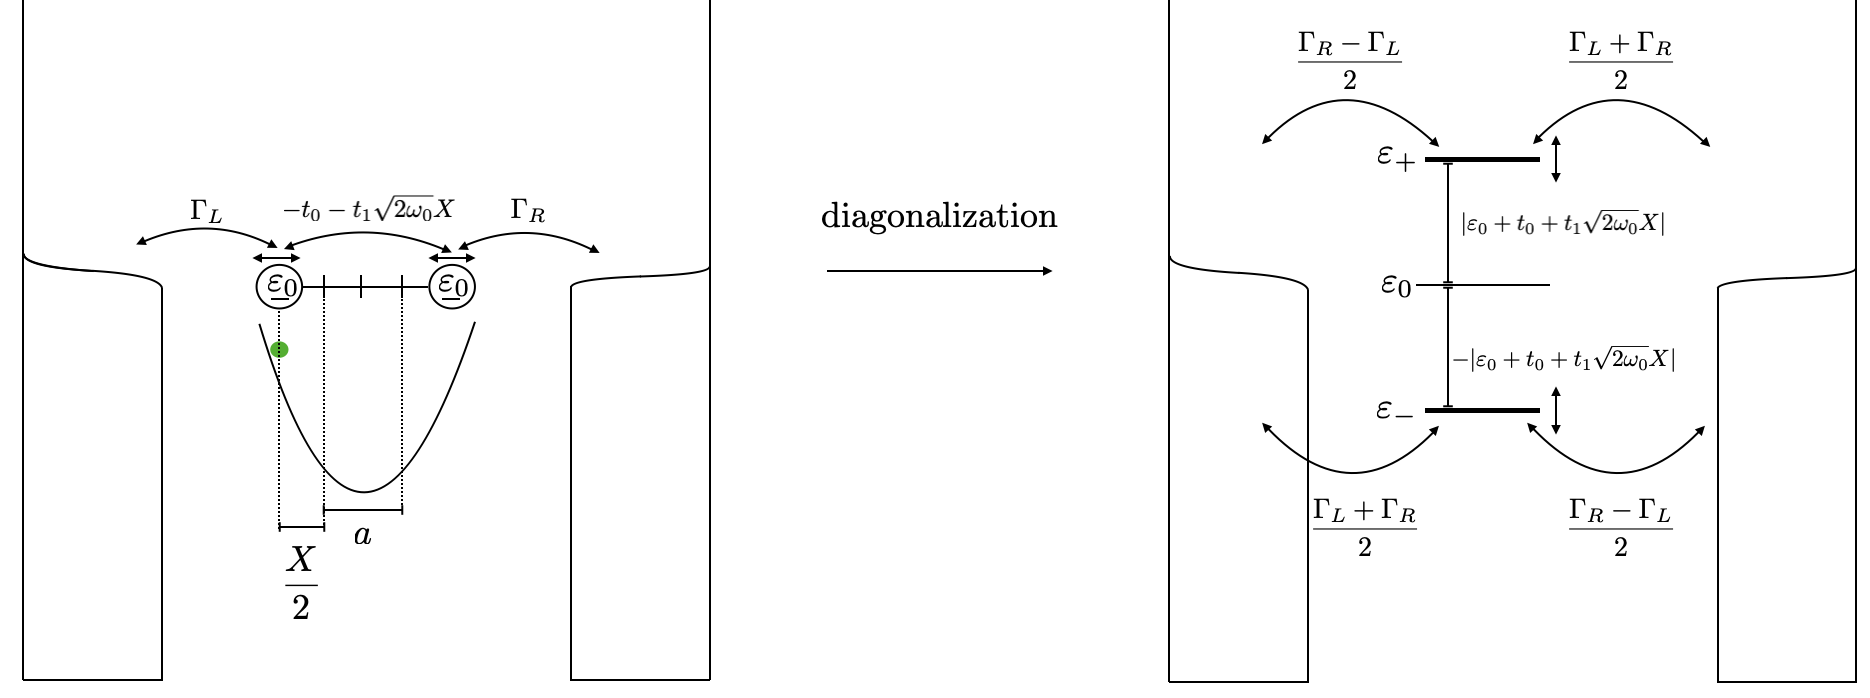
\includegraphics[width=1.0\textwidth]{figs/Schematic_Peierls_diagonalization.png}
	\caption{Schematic of the two-site classical Peierls model in the site-basis (left) and the energy-eigenbasis (right).}\label{fig:Schematic_Peierls_transformed}
\end{figure}\\
The reduced density matrix at time $t$ in this basis is then
\begin{equation}
	\tilde{\rho}(t) = \begin{pmatrix}
	\vert c_-(t)\vert^2 &  c_-^{\phantom{*}}(t)c_+^*(t) \\
	c_+^{\phantom{*}}(t)c_-^*(t) & \vert c_+(t)\vert^2 
	\end{pmatrix}.
\end{equation}
Populating a state $\vert\psi_\pm\rangle$ produces a quantum force on the vibration
\begin{align}
	F(t) &\sim -\tr{\rho(t)\partial_X H_\mathrm{el-ph}} \\
	&= -\tr{\tilde{\rho}(t)\partial_X \tilde{H}_\mathrm{el-ph}}\\
	&= -\sqrt{2\omega}t_1\tr{\tilde{\rho}(t) (c_-^\dagger c_-^\pdagger - c_+^\dagger c_+^\pdagger)} = \sqrt{2\omega}t_1 (\vert c_+\vert^2 - \vert c_-\vert^2).\\
\end{align}
From this expression it is clear that a coherence between eigenstates in $\rho(t)$ does not produce a force on the vibration. The force depends only on the population difference of the two molecular electronic eigenstates. The $\sim$ sign is there because the force also contains a harmonic potential part, which is not relevant here because we want to know the effect coming from the electrons alone. This force (together with the harmonic contribution) will drive the vibration to a new momentum and position
\begin{align*}
	P(t+\dif t) &\approx  P(t) - \dif t (\sqrt{2\omega}t_1(\vert c_-(t)\vert^2 - \vert c_+(t)\vert^2 ) + \omega^2 X(t)) \\
	X(t+\dif t) &\approx X(t) + \dif t P(t).
\end{align*}
The new position $X(t+\dif  t)$ enters the Hamiltonian to yield $H(t+\dif t)$, and thus leads to new changes in $\rho(t+\dif t)$ in the next time-step. This cycle repeats itself until the simulation is finished. Since both the coupling to the leads and the vibrational motion leads to changes in $\rho(t)$, it is beneficial to disentangle the effects from each other coming from these two origins. This can be achieved in different ways: 
\begin{itemize}
	\item Investigate dynamics for $t_1=0$ and compare to with vibronic coupling
	\begin{itemize}
		\item This shows purely electronic effects
		\item We do not learn anything about influence of electrons on vibrations and vice versa
	\end{itemize}
	\item Solve HEOM for $\rho(t)$ under $H(X(t))$, but classical EOM assuming $t_1=0$
	\begin{itemize}
		\item Action of vibration on electronic dynamics
		\item We do not learn anything about the back-reaction of the electrons on the vibration
	\end{itemize}
	\item Solve HEOM for $\rho(t)$ assuming $t_1 = 0$, but classical EOM under influence of electrons
	\begin{itemize}
		\item Action of electron on vibrational dynamics 
		\item We do not learn anything about the back-reaction of the vibration on the electrons
	\end{itemize}
\end{itemize}
\section{Simplification of problem: Slow charge dynamics}\label{sec:SimpleParams}
The problem can be simplified by setting the parameters to
\begin{align*}
	\varepsilon_0 &= \SI{0}{\milli\electronvolt}\\
	\omega_0 &= \SI{0.1}{\electronvolt}\\
	t_0 &= \SI{2}{\electronvolt}\\
	t_1 &= \SI{0.2}{\electronvolt}\\
	\Gamma &= \SI{10}{\milli\electronvolt}\\
	T &= \SI{5}{\milli\electronvolt}.
\end{align*}
Setting the temperature to roughly $\SI{60}{\kelvin}$ and the system-lead coupling $\Gamma=\SI{10}{\milli\electronvolt}$ ensures that thermal broadening is suppressed, but the states are only broadened by the coupling to the leads. 
The two levels are separated by $2\varepsilon_+$, which is proportional to $t_0$. Hence, setting $t_0/\Gamma = 200$ leads to well-resolved and relatively narrow conductance peaks at $V=2\varepsilon_\pm$. From the perspective of dynamics, $\Gamma$ is the bottleneck of all processes with an onset of steady-state expected at $\tau_\mathrm{el}\sim\Gamma^{-1}\approx \SI{25}{\femto\second}$ (hopping takes place on a time-scale of $\sim \SI{120}{\atto\second}$), while the vibrational time-scale is $\tau_\mathrm{ph}\sim 2\pi\omega^{-1} \approx \SI{15}{\femto\second}$. Hence, the the vibration can readjust dynamically to the charge dynamics and we can investigate the validity of the previous analysis. 
Shifting the on-site energy to zero simplifies the analysis when we apply a voltage. The choice of $T,\Gamma,\varepsilon_0$ and $t_0$ altogether ensures that in equilibrium only the state $\vert\psi_-\rangle$ below Fermi level is occupied. 
However, $\Gamma/T=2$ is rather large an higher-order transport processes, such as co-tunneling, are expected to be present.
An occupancy of both states is only possible when a finite voltage $V\gtrapprox 2\varepsilon_\pm$ (a voltage smaller than $2\varepsilon_\pm$ is also fine if the states are sufficiently broadened) is applied. For $t_1=0$, the I-V curve is shown in \cref{fig:IV_L2_t1_0}. 
\begin{figure}[!h]
	\centering
	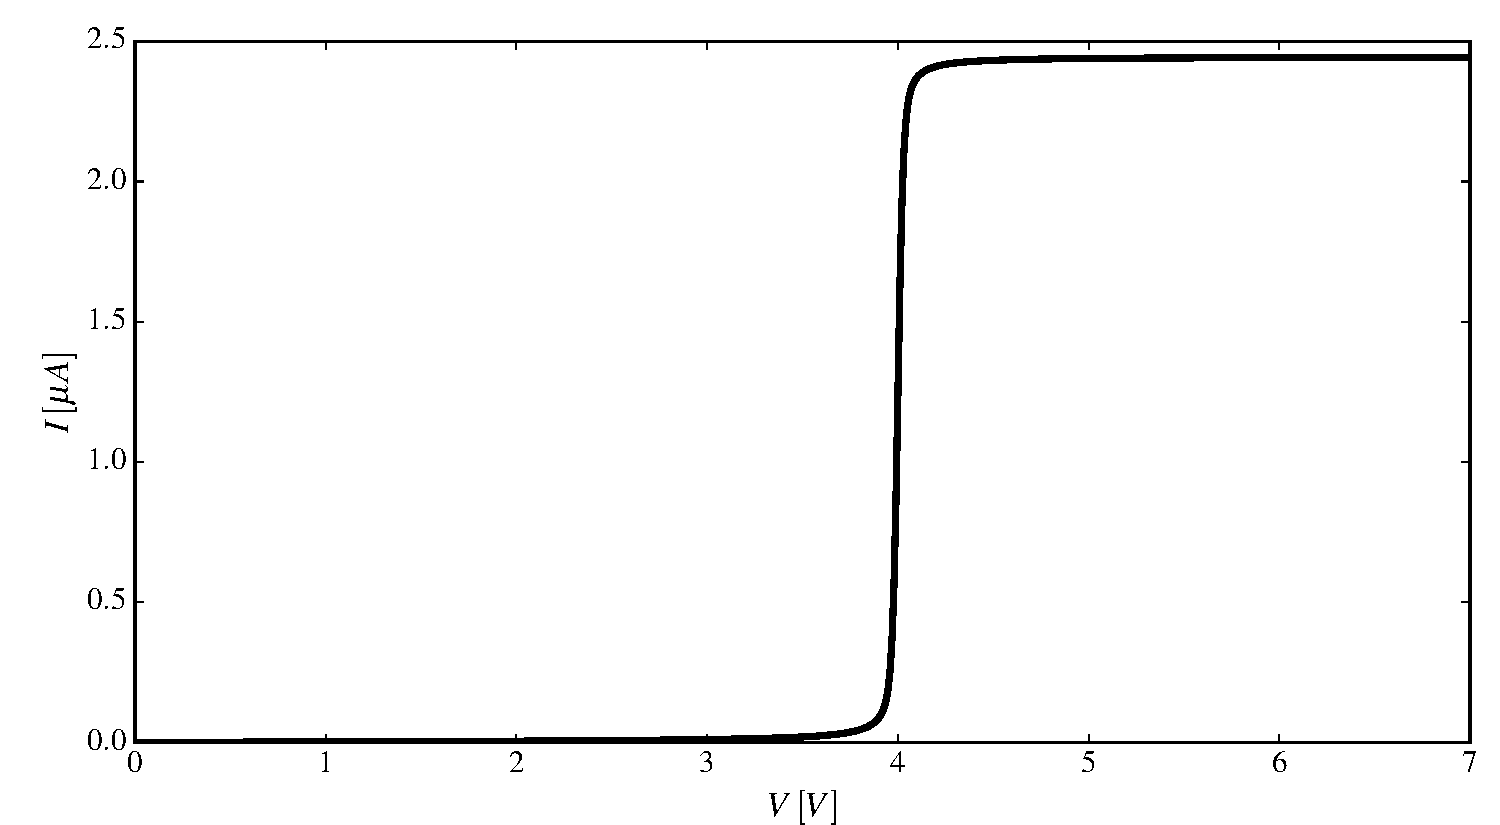
\includegraphics[width=1.0\textwidth]{figs/Peierls_L2_noPh_IV.pdf}
	\caption{I-V curve for the parameters given above and $t_1=\SI{0}{\electronvolt}$.}\label{fig:IV_L2_t1_0}
\end{figure}\\
\subsection{Single-trajectory results}
\indent We set the voltage to $V=\{0,4,7\}\, \mathrm{V}$ which represent the three different voltage regimes (without electron-vibrational coupling): No electronic levels in the bias window, chemical potential on resonance with the levels, and both levels in the bias window. The symmetrized current is shown in \cref{fig:I_t_L2_N_params} and the phonon energy in \cref{fig:Eph_t_L2_N_params}. Further, \cref{fig:ES_t_L2_N_params} shows the population of the eigenstates $\vert\psi_\pm\rangle$ and \cref{fig:ELD_t_L2_N_params} shows the instantaneous eigenenergies $\varepsilon_\pm$ under the influence of vibrational dynamics corresponding to the different voltages. 
These figures show a single trajectory with the same initial condition as used in \cref{fig:I_t_L2_F_params,fig:Eph_t_L2_F_params}.
%The most striking effects are for $V=\SI{4}{\volt}$. There, the current strongly oscillates back and forth, the vibrational energy increases linearly with time, the eigenstate population oscillates strongly and the vibrational displacement attains a value large enough such that the eigenlevels $\varepsilon_\pm$ cross. 
\begin{figure}[!h]
	\centering
	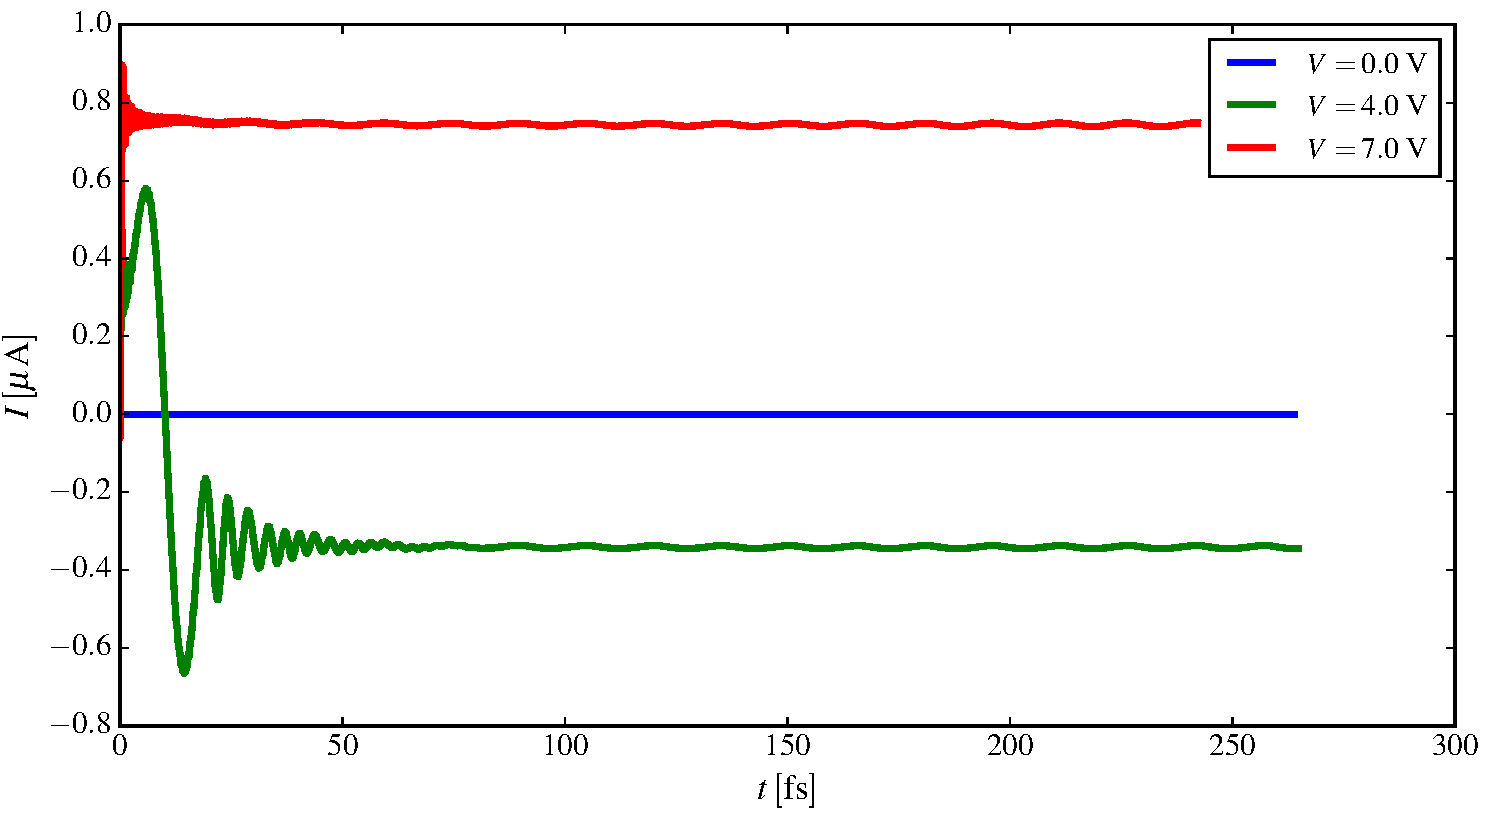
\includegraphics[width=1.0\textwidth]{figs/Peierls_L2_NewParams_Vvar_currents.pdf}
	\caption{Symmetrized current for the parameters listed above.}\label{fig:I_t_L2_N_params}
\end{figure}
\begin{figure}[!h]
	\centering
	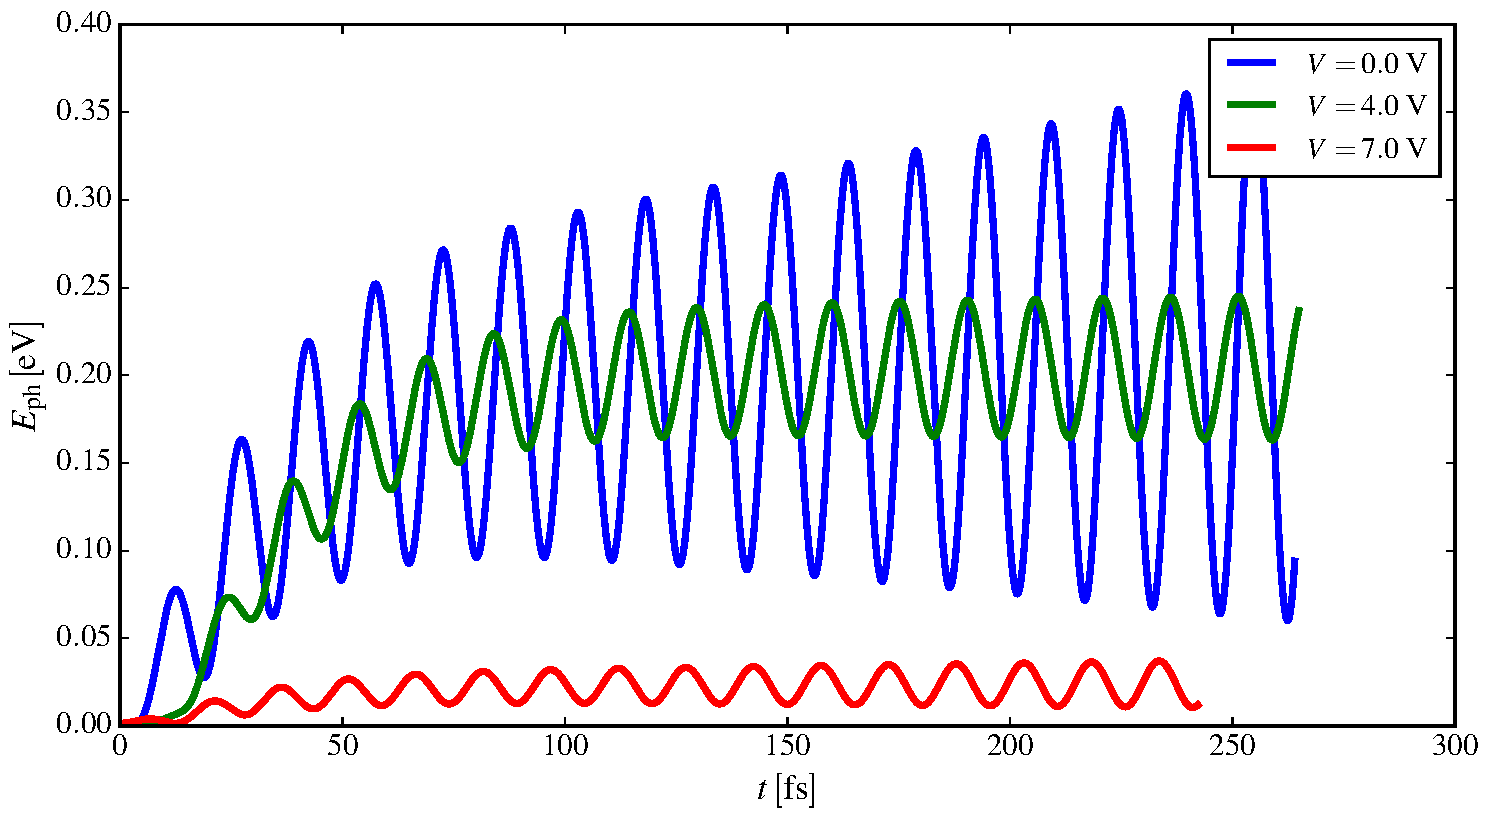
\includegraphics[width=1.0\textwidth]{figs/Peierls_L2_NewParams_Vvar_phonons.pdf}
	\caption{Phonon energy dynamics for the parameters listed above.}\label{fig:Eph_t_L2_N_params}
\end{figure}
\begin{figure}[!h]
	\centering
	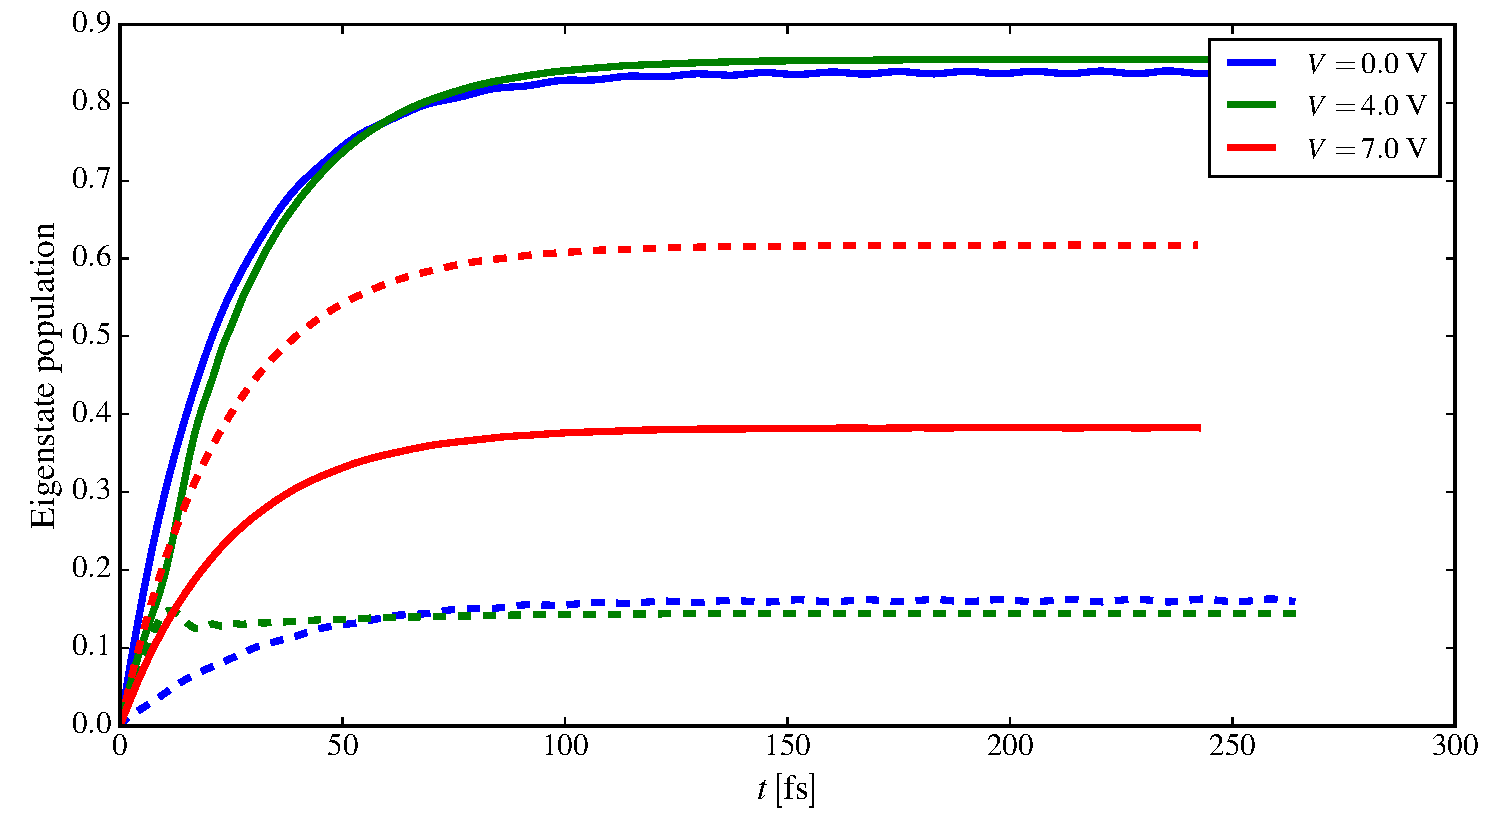
\includegraphics[width=1.0\textwidth]{figs/Peierls_L2_NewParams_Vvar_ES.pdf}
	\caption{Eigenstate population dynamics. The full line shows the population of lower state $\vert \psi_-\rangle $, the dashed one the population of upper state $\vert \psi_+\rangle$.}\label{fig:ES_t_L2_N_params}
\end{figure}
\clearpage
\begin{figure}[!h]
	\centering
	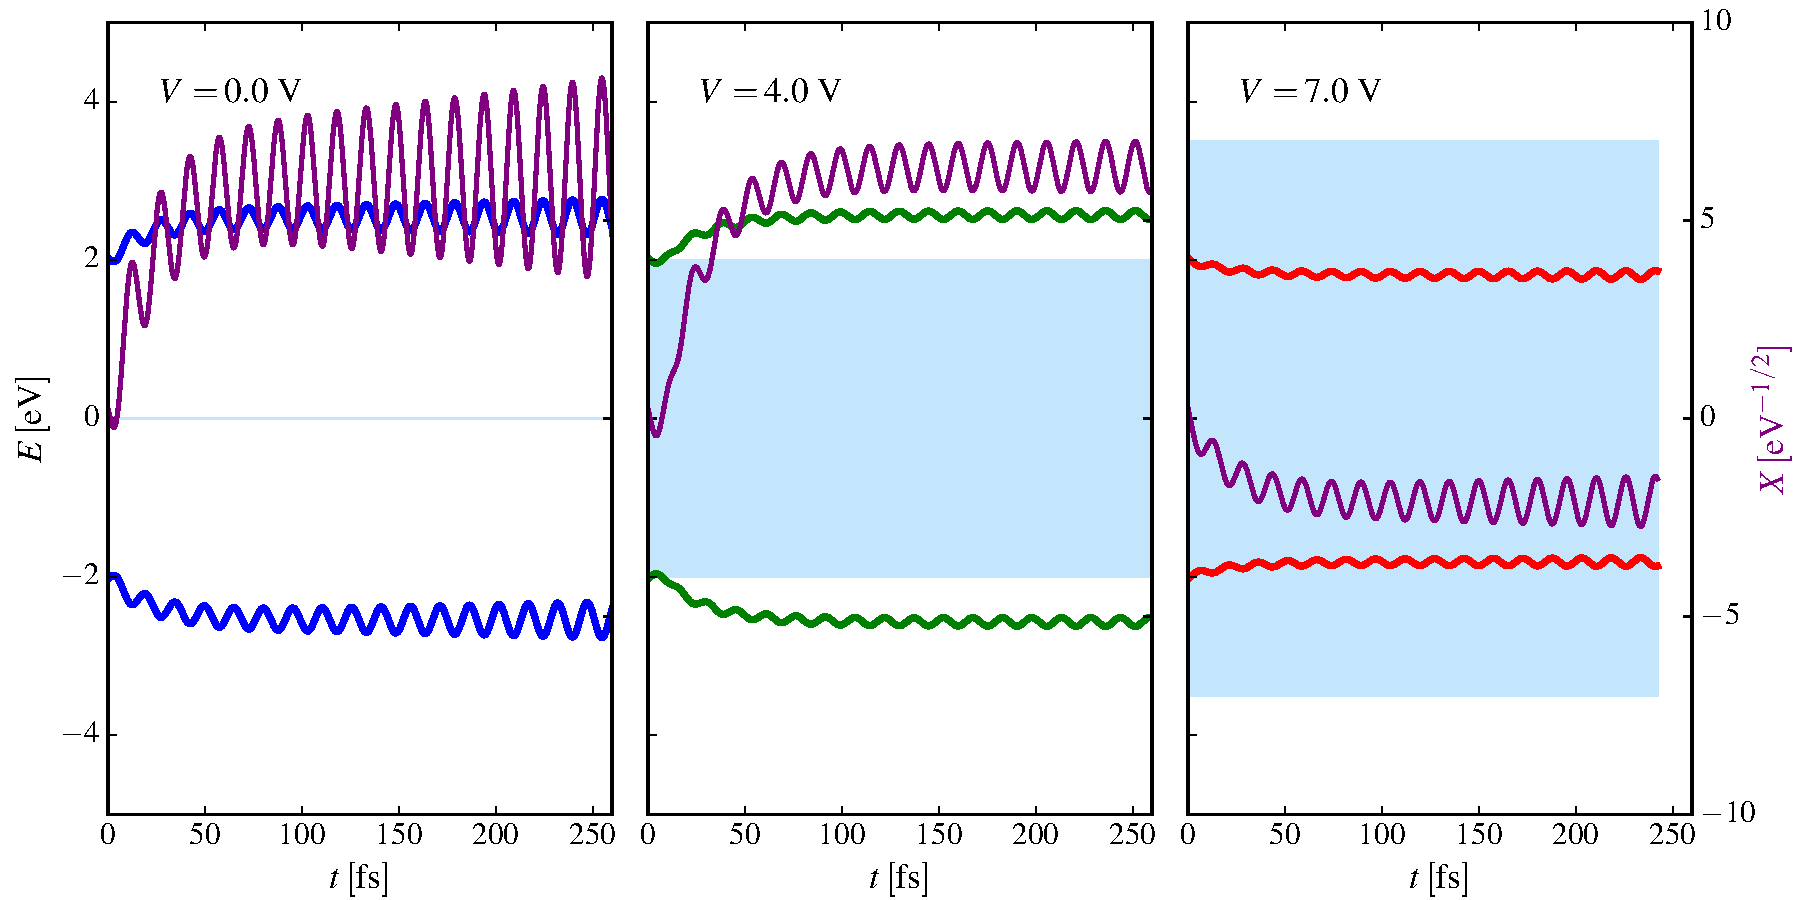
\includegraphics[width=1.0\textwidth]{figs/Peierls_L2_NewParams_EL_ParVar_Ph.pdf}
	\caption{Instantaneous eigenlevels under vibrational dynamics.}\label{fig:ELD_t_L2_N_params}
\end{figure}
\subsection{Averaged result}
\begin{figure}[!h]
	\centering
	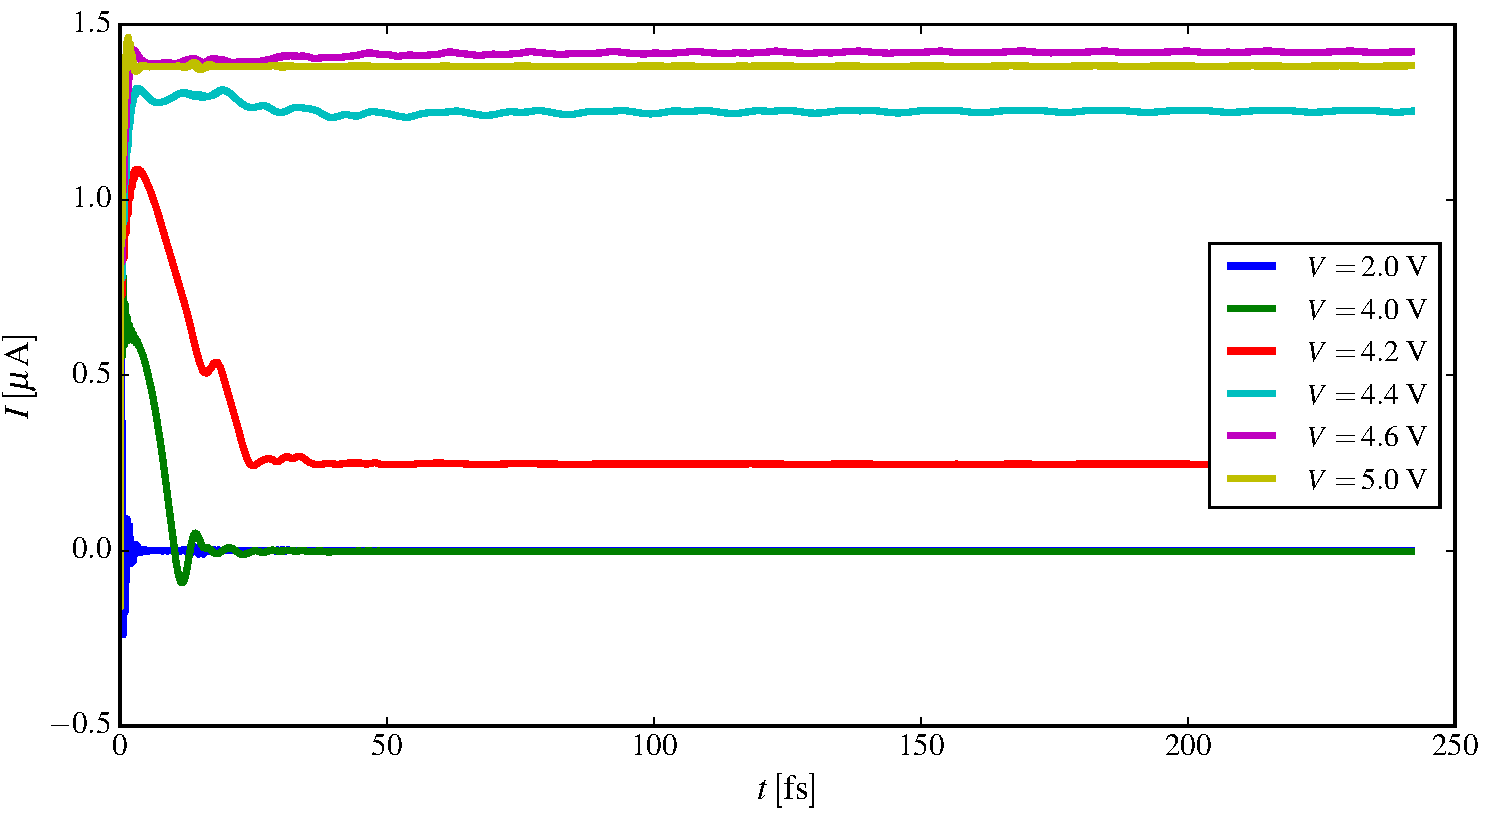
\includegraphics[width=1.0\textwidth]{figs/Peierls_L2_NewParams_Vvar_avg_currents.pdf}
	\caption{Symmetrized current for the parameters listed above, averaged over 6000 trajectories.}\label{fig:I_t_L2_avg_N_params}
\end{figure}
\begin{figure}[!h]
	\centering
	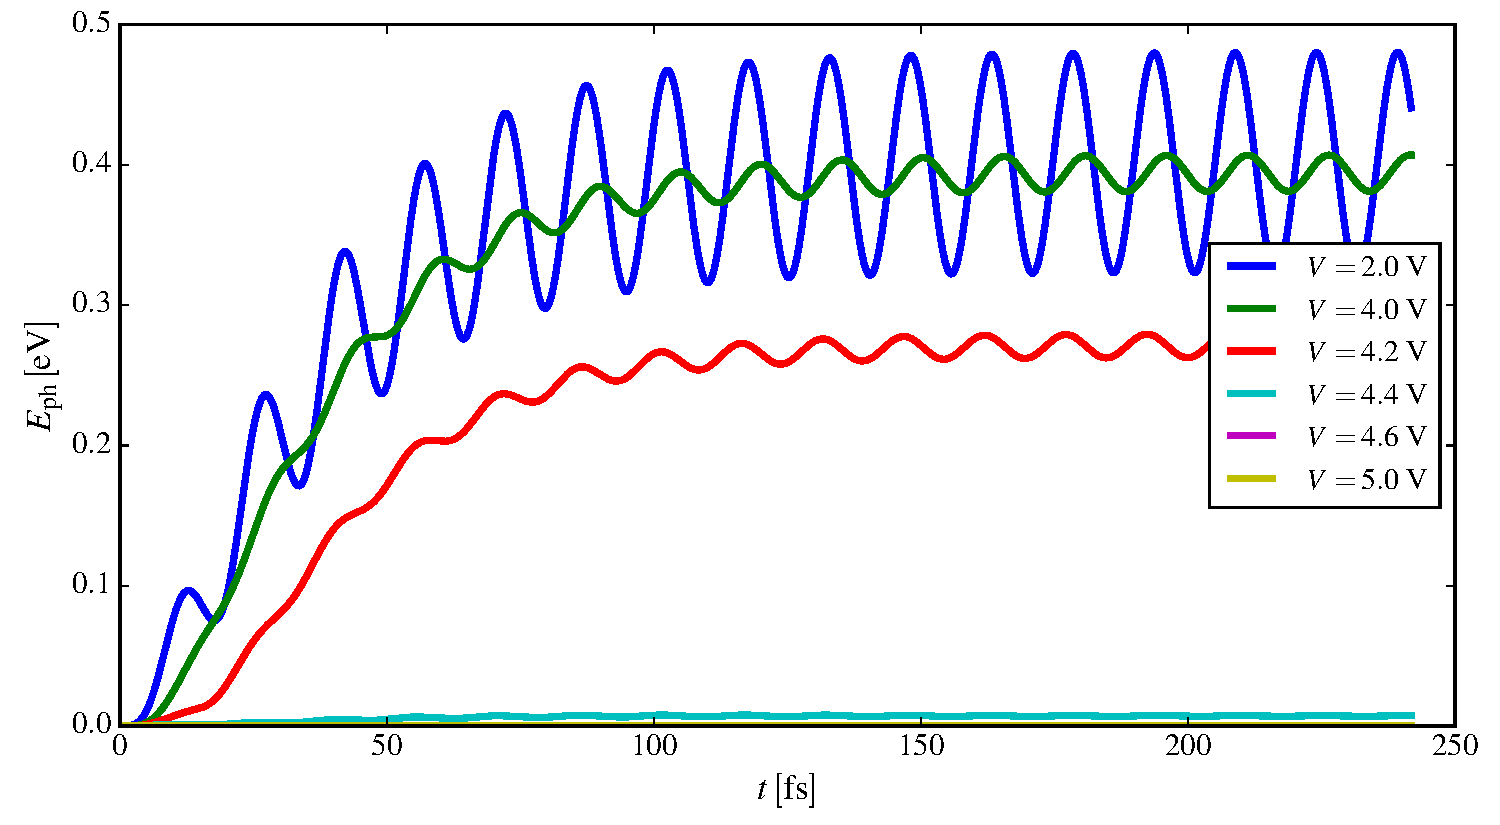
\includegraphics[width=1.0\textwidth]{figs/Peierls_L2_NewParams_Vvar_avg_phonons.pdf}
	\caption{Phonon energy dynamics for the parameters listed above, averaged over 6000 trajectories.}\label{fig:Eph_t_L2_avg_N_params}
\end{figure}
\begin{figure}[!h]
	\centering
	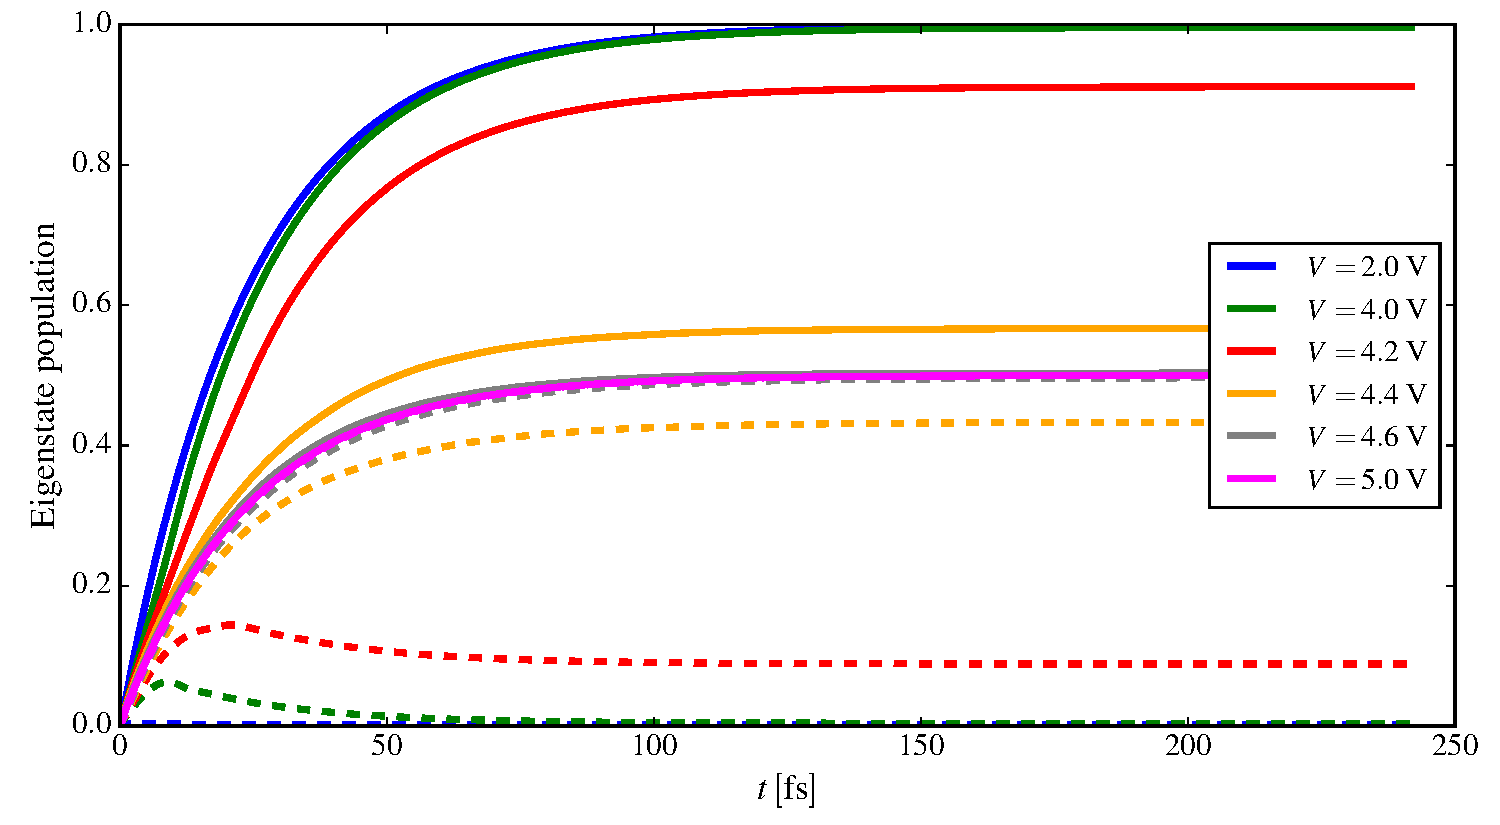
\includegraphics[width=1.0\textwidth]{figs/Peierls_L2_NewParams_Vvar_avg_ES.pdf}
	\caption{Eigenstate population dynamics. The full line shows the population of lower state $\vert \psi_-\rangle $, the dashed one the population of upper state $\vert \psi_+\rangle$. The results are averaged over 6000 trajectories.}\label{fig:ES_t_L2_avg_N_params}
\end{figure}
\clearpage
\begin{figure}[!h]
	\centering
	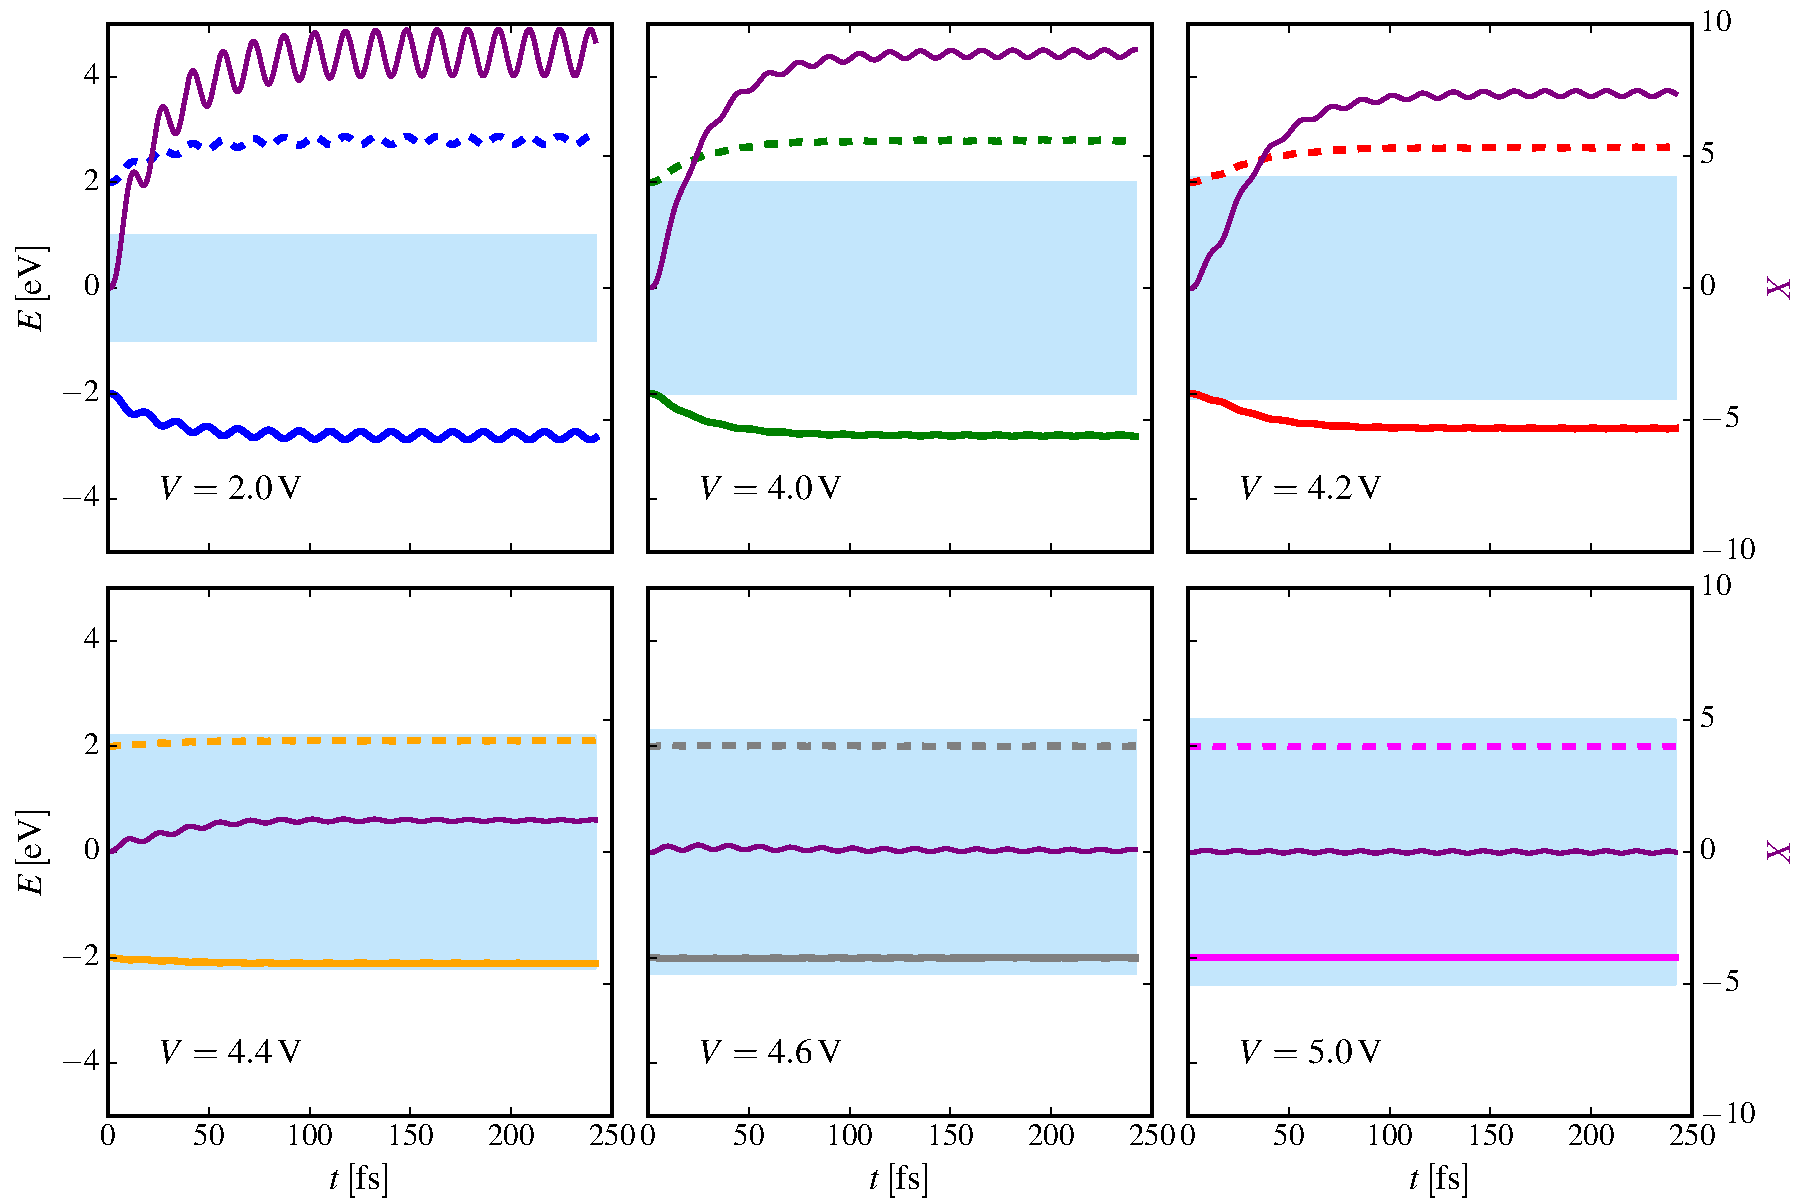
\includegraphics[width=0.9\textwidth]{figs/Peierls_L2_NewParams_EL_ParVar_Ph_avg.pdf}
	\caption{Instantaneous eigenlevels under vibrational dynamics, averaged over 6000 trajectories.}\label{fig:ELD_t_L2_avg_N_params}
\end{figure}
\begin{figure}[!h]
	\centering
	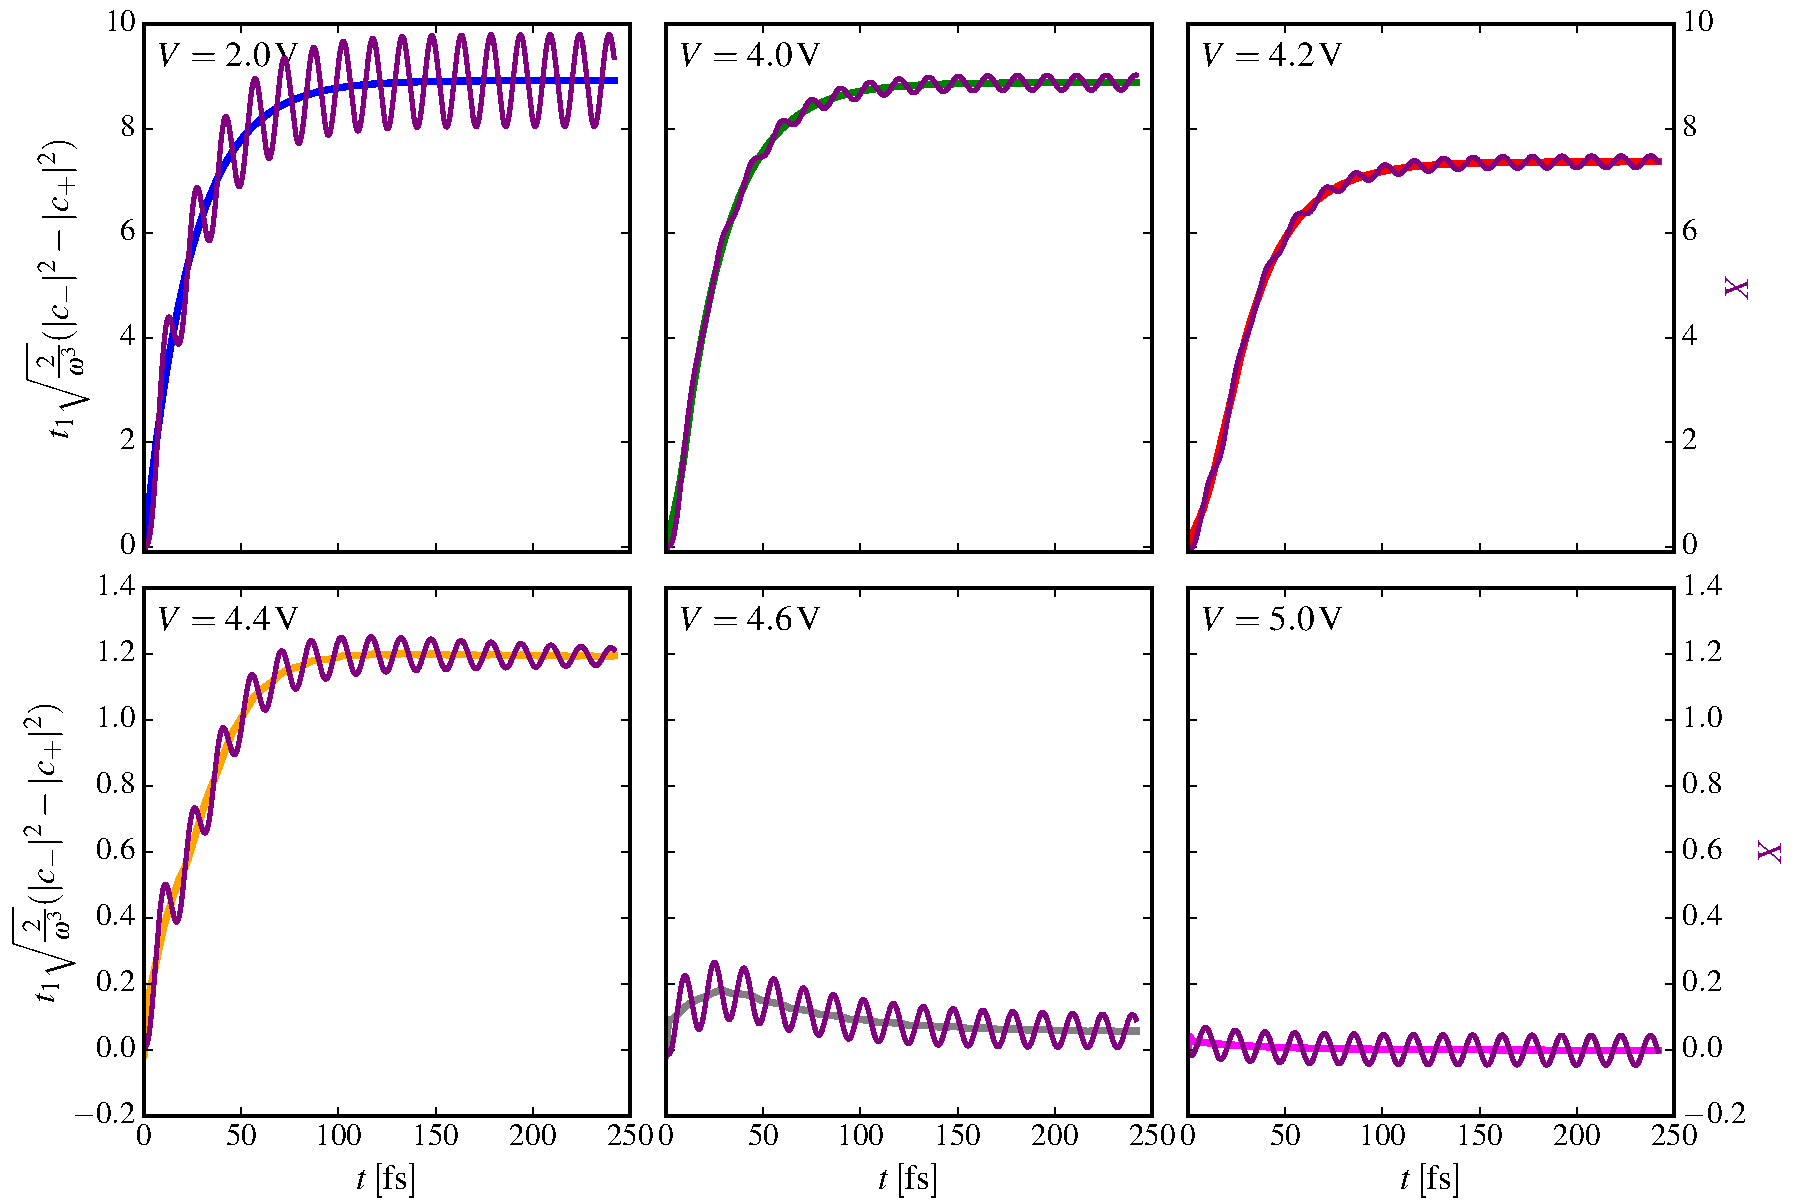
\includegraphics[width=0.9\textwidth]{figs/Peierls_L2_NewParams_EL_ES_ParVar_Ph_avg.pdf}
	\caption{Minimum of mean-field vibrational potential energy (\cref{eq:VibPotentialMF_minimum}), obtained from the instantaneous eigenstate population difference $\vert c_-\vert^2-\vert c_+\vert^2$, and vibrational position $X$.}\label{fig:EL_ESD_t_L2_avg_N_params}
\end{figure}

\clearpage
\section{Analysis of the problem (II) and answers}
\begin{itemize}
	\item[Q:] Why does the current drop down to zero for $V=\SI{4}{\electronvolt}$?
	\item[A:] Check out the energy-eigenlevels for $V=\SI{4}{\electronvolt}$ in \cref{fig:ELD_t_L2_N_params,fig:ELD_t_L2_avg_N_params}. Without electron-vibrational coupling, both levels are inside the bias window and a current can flow through the system. Initially, the mean vibrational position is $\langle X_0\rangle = 0$, and hence the energy-gap is not modified by the vibronic coupling initially.
	Due to the coupling to the leads, the eigenstate populate increases. The modified vibrational potential energy is then
	\begin{align}
		U(X) &= \frac{\omega^2X^2}{2} - \sqrt{2\omega}t_1 X(\vert c_-\vert^2-\vert c_+\vert^2),\label{eq:VibPotentialMF}\\
		&= \frac{\omega^2}{2}(X+a)^2 + b \\
		b &= -\frac{\omega^2}{2}a^2\\
		a &= -t_1 \sqrt{\frac{2}{\omega^3}} (\vert c_-\vert^2-\vert c_+\vert^2)
	\end{align}  
	The potential $U(X)$ is shown in \cref{fig:U(X)_MF} for an unoccupied molecule (blue line), the upper level fully occupied and the lower unoccupied (green line), the lower fully occupied and the upper unoccupied (red line), and both levels equally occupied (dashed teal line). 
	\begin{figure}[!h]
		\centering
		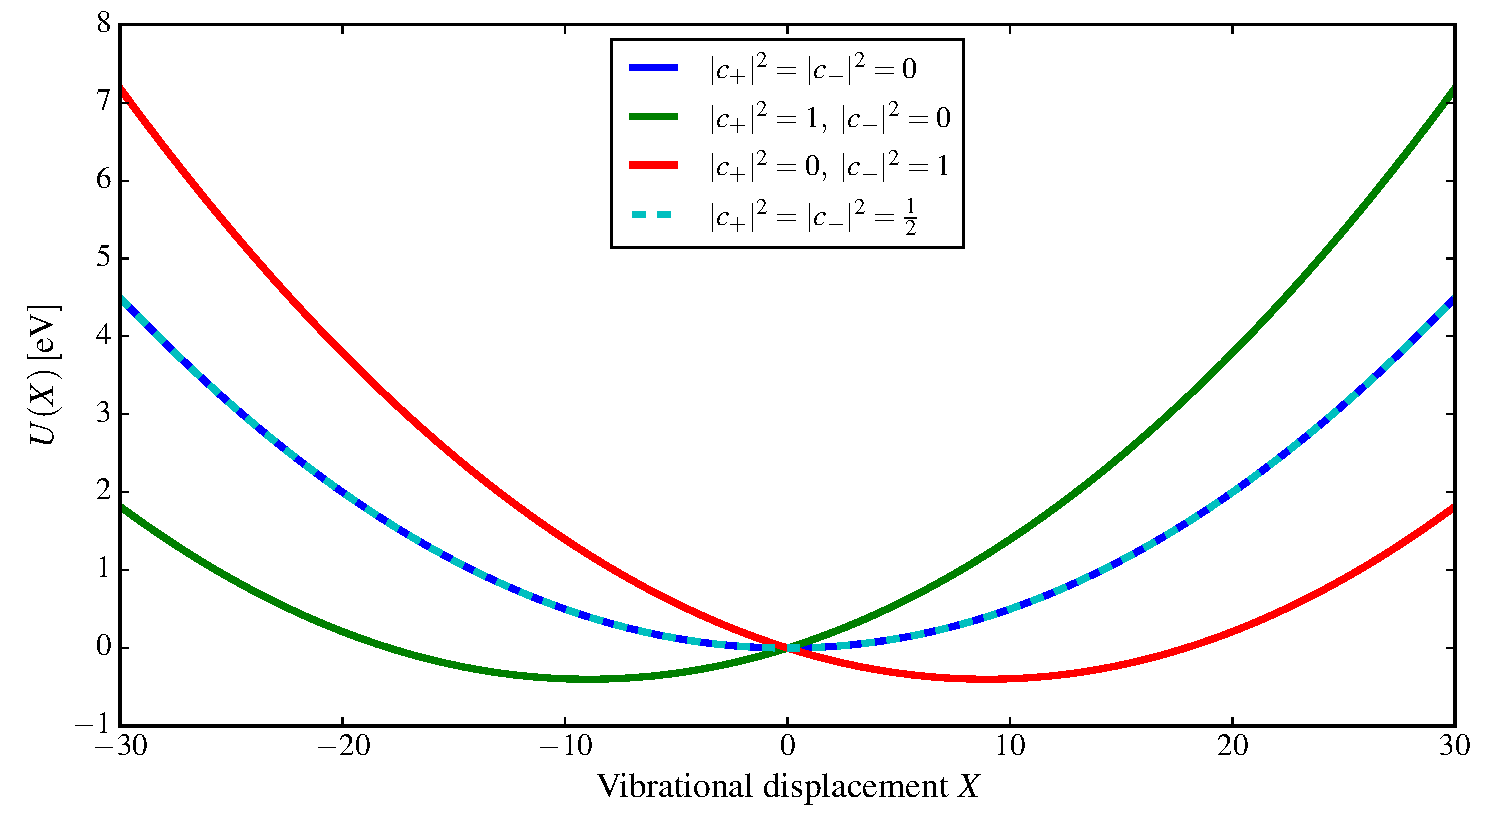
\includegraphics[width=0.9\textwidth]{figs/L2_Peierls_MF_potential.pdf}
		\caption{Mean-field vibrational potential energy $U(X)$ for selected electronic populations.}\label{fig:U(X)_MF}
	\end{figure}\\
	For $V=\SI{4}{\volt}$ after $\sim \SI{150}{\femto\second}$, the molecule is approximately fully occupied in its lower state and unoccupied in the upper state (\cref{fig:ES_t_L2_avg_N_params}, green lines). In this situation, the minimum of $U(X)$ is (with $\omega=\SI{0.1}{\milli\electronvolt}$, $t_1=\SI{0.2}{\electronvolt}$) at $X=\sqrt{80}\approx 8.94$. In \cref{fig:ELD_t_L2_avg_N_params} one can see that $X$ oscillates around $8.9$, which is in good agreement with the analytical prediction. 
	Another example is $V=\SI{5.0}{\volt}$, for which both eigenstates are populated approximately equally. The expected minimum is thus at $X=0$, which agrees with the numerical value around which $\langle X\rangle$ oscillates (\cref{fig:ELD_t_L2_avg_N_params}).
	The electronic populations, however, do not change instantaneously, but on a time-scale dictated by the coupling to the leads $\Gamma$. The vibrational potential energy therefore changes smoothly with time. When the electronic steady-state is reached, the vibrational mode oscillates around the minimum of the potential with $\langle X\rangle >0$. Since the gap 
	\begin{equation}
	\Delta\varepsilon = \varepsilon_+-\varepsilon_- = 2\vert t_0+\sqrt{2\omega}t_1X\vert \label{eq:GapXDep}
	\end{equation}
	is proportional to $X$, the levels are on average pushed outside of the bias window (see \cref{fig:ELD_t_L2_avg_N_params}), which results in no available open transport channels and thus to a vanishing current. From the time-evolution of the current shown in \cref{fig:I_t_L2_F_params_avg} one can see that the current reaches a finite value after $\sim \SI{10}{\femto\second}$, which is consistent with the fact that the electronic time-scale in the molecule is  $\tau_\mathrm{el}\sim \SI{120}{\atto\second}$. The current drops then to zero, because the vibrational dynamics is activated (from the vibrational frequency one gets $\tau_\mathrm{ph}\approx \SI{15}{\femto\second}$), leading to a change in the electronic energies as discussed above. Since the states have been partially populated within the first $\SI{10}{\femto\second}$, and the energy of the states is above the Fermi-level of the leads, there is a current of electrons from the molecule into the leads. This scenario is schematically depicted in \cref{fig:Current_processes_N}.
	In particular, $X$ has to be at least 
	\begin{equation}
		X > \frac{1}{t_1\sqrt{2\omega}}\left(\frac{V}{2}-t_0\right)
	\end{equation}
	in order to push the levels outside of the bias window for a fixed voltage $V$.
	In this case, assuming the levels are never fully occupied, there is a current from the right lead into the lower level and a current from the upper level into both lead (hence $I<0$, as seen for the single trajectory in \cref{fig:I_t_L2_N_params}). 
	\begin{figure}[!h]
		\centering
		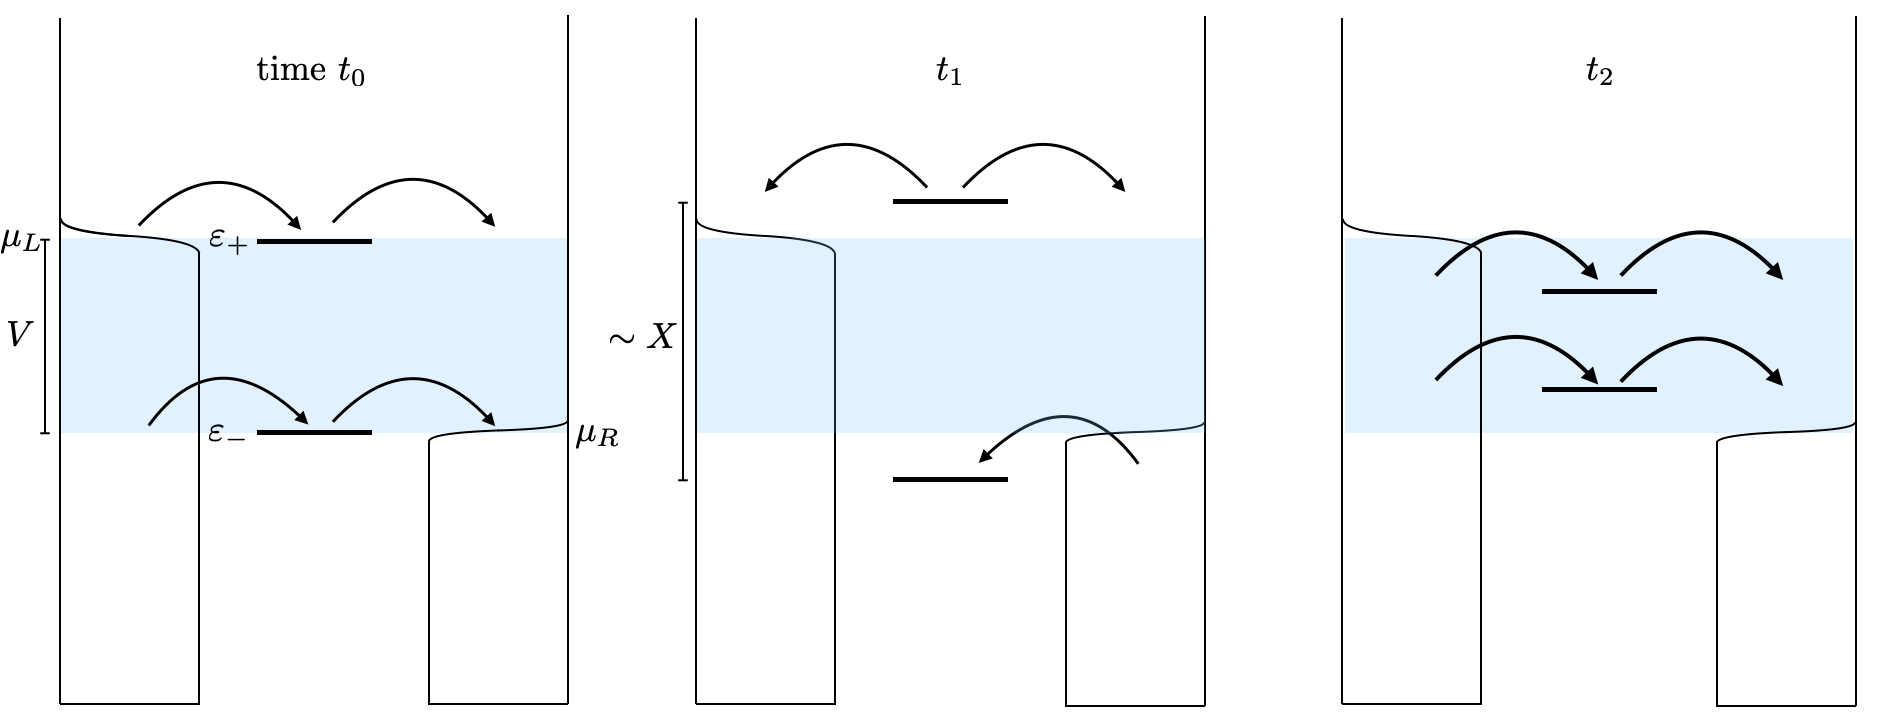
\includegraphics[width=0.9\textwidth]{figs/Peierls_L2_current_processes_SimpleParams_V4.png}
		\caption{Resonant electronic processes for $V=\SI{4}{\electronvolt}$ for $X=0$ ($t_0$), $X>0$ ($t_1$), and $X<0$ ($t_2$). The instantaneous electronic energies are depicted by black horizontal bars. The arrows denote the direction of charge current. For $t_0$ both levels are at the edges of the bias window, at $t_1$ both levels are outside of the bias window (levels are assumed to be populated) and at $t_2$ both are inside the bias window.  
		}\label{fig:Current_processes_N}
	\end{figure}
	\item[Q:] Why does the vibrational mode move to a new equilibrium position for low voltages (meaning, the molecular levels are not in the bias window)?
	\item[A:] Since $\varepsilon=\SI{0}{\electronvolt}$, for these voltages only the lower state $\vert \psi_-\rangle$ gets occupied as it is below Fermi-level. With the same argument as given in the previous answer, the population of the lower level will reach $1$ while the upper level remains unoccupied. For this case, the potential energy $U(X)$ is shown in \cref{fig:U(X)_MF} by the red curve. The vibrational mode will thus follow the potential energy surface to its new minimum. 
	\item[Q:] If both levels are in the bias window for $V=\SI{7}{\electronvolt}$, why does the current oscillate slightly?
	\item[A:] The oscillation comes from the vibrations. However, because voltage is large enough so that both levels are inside the bias window, this cannot be the full explanation. Actually, there are two effects. First, the vibrational mode oscillates around an equilibrium position $X_0> 0$, which increases the energy gap and and pushes the levels closer to the edges of the bias window. 
	Second, the integrated spectral density decreases whenever $X$ increases because a small part of the electronic spectral density is pushed out of the bias window. 
	\item[Q:] What is the frequency of the oscillations?
	\item[A:] It is $\omega\approx \omega_0$ but slightly below, similar to the driven harmonic oscillator.
	\item[Q:] What determines the vibrational oscillation amplitude?
	\item[A:] To answer this question, consider following cases with slight changes in the parameters (schematically depicted in \cref{fig:Peierls_L2_SimpleParams_Schematic_cases}):
	\begin{itemize}
		\item[(i)] Both levels can enter and leave the bias window due to vibrational dynamics
		\begin{itemize}
			\item Chemical potentials resonant with eigenlevels $\mu_L=\varepsilon_+$, $\mu_R= \varepsilon_-$
			\item The levels can enter and leave the bias window as $X$ varies
			\item Same parameters as above, $V=2t_0 = \SI{4}{\volt}$
		\end{itemize}  
		\item[(ii)] Both levels are inside the bias window but cannot leave it due to vibrational dynamics
		\begin{itemize}
			\item Chemical potentials not resonant with eigenlevels, but both levels inside bias window $\mu_L>\varepsilon_+$, $\mu_R< \varepsilon_-$
			\item A very large $X$ is necessary to push the levels outside of the bias window
			\item Same parameters as above, $V=\SI{20}{\volt}$,
		\end{itemize}
		\item[(iii)] Transport channel through lower level blocked, but upper can enter and leave bias window
		\begin{itemize}
			\item Left chemical potential is resonant with the upper level $\mu_L=\varepsilon_+$, but right chemical potential not resonant $\mu_R>\varepsilon_+$. 
			\item The vibrational mode can push the upper level outside the bias window, but the lower one cannot enter the bias window.
			\item Parameters: $\varepsilon_0 = -\SI{1}{\electronvolt}$, $V=\SI{2}{volt}$
		\end{itemize}
		\item[(iv)] Transport through lower level blocked, but upper level cannot leave the bias window 
		\begin{itemize}
			\item The upper level is inside the bias window and the lower one is outside.
			\item Variation of $X$ does not push upper level outside the bias window.
			\item Parameters: $\varepsilon_0 = -\SI{2}{\electronvolt}$, $V=\SI{2}{\volt}$
		\end{itemize}
		\item (v) Same as case (iii) but now the lower level is inside the bias window and the upper one outside and (vi) same as (iv) but now the lower level is inside the bias window and the upper one outside
		\begin{itemize}
			\item Transport invariant under a global energy shift
			\item Cases will not be considered, as due to this invariance the symmetrized current and the vibrational dynamics is expected to be identical to the other
			cases
			\item However, the left and right currents, individually, may vary because the upper and lower level couple with an alternating sign to the vibrational position
		\end{itemize}
	\end{itemize}
	\begin{figure}[!h]
		\centering
		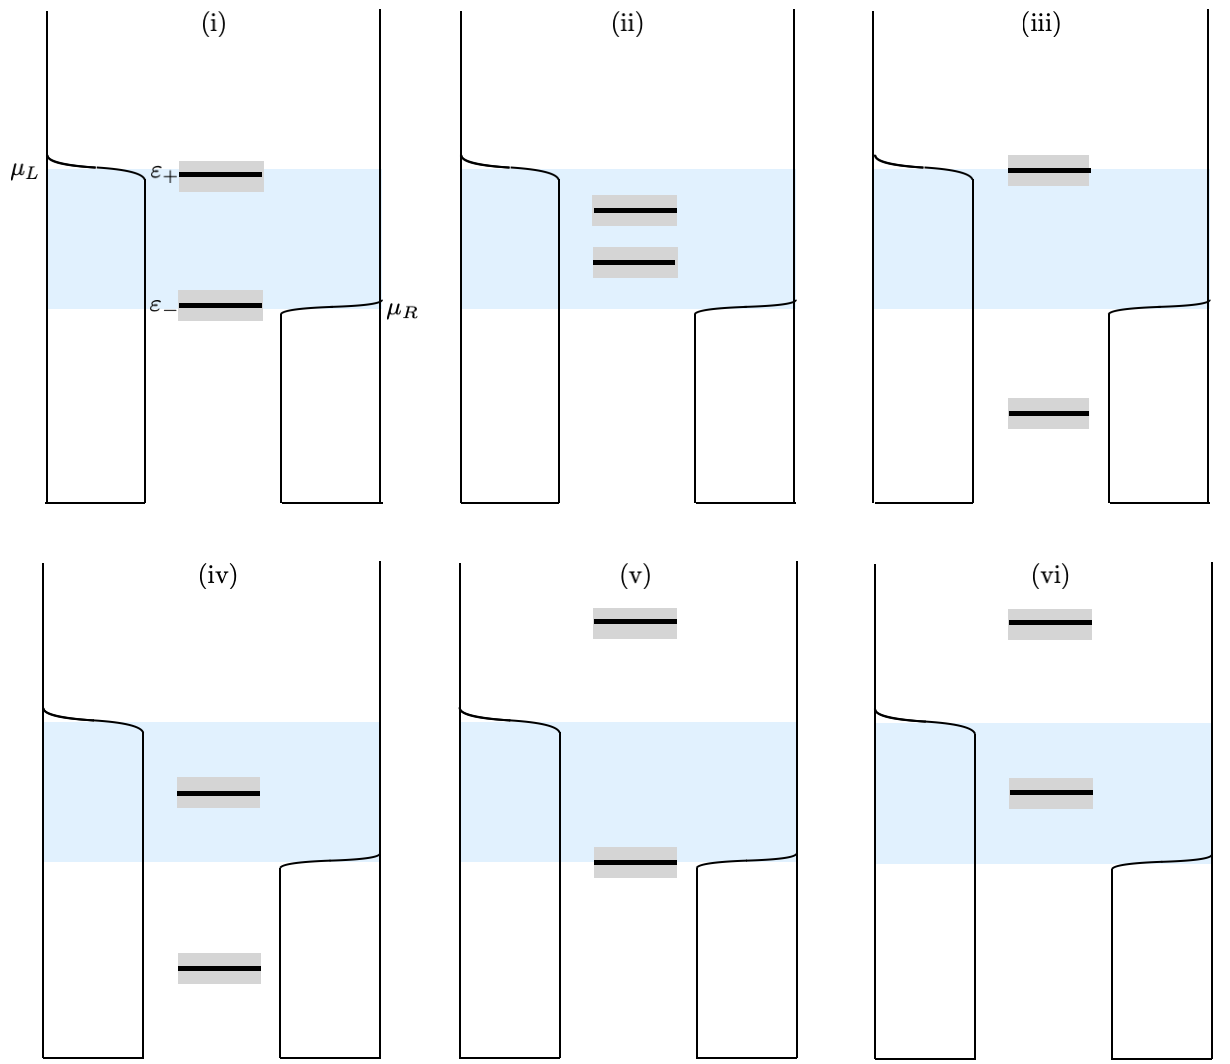
\includegraphics[width=0.8\textwidth]{figs/L2_Peierls_SimpleParams_schematic_cases.png}
		\caption{Schematics of the cases discussed above. The light blue box indicates the bias window and the gray boxes indicate the typical variation of the levels position due to vibrational dynamics.}\label{fig:Peierls_L2_SimpleParams_Schematic_cases}
	\end{figure}
	As in the previous analysis, the symmetrized current is shown in \cref{fig:Peierls_L2_SimpleParams_Cases_currents}, the vibrational energy in \cref{fig:Peierls_L2_SimpleParams_Cases_phonons}, the population of eigenstates in \cref{fig:Peierls_L2_SimpleParams_Cases_ES}, and \cref{fig:Peierls_L2_SimpleParams_Cases_El_vib} shows the eigenenergies and the vibrational position (purple line) for the cases discussed above. The vibrational energy increases linearly only in case (i). In all other cases, the vibrational energy saturates (while oscillating). Also, in case (i) the current and the populations of the eigenenergies strongly oscillate. This does not happen in the other cases, except for case (iii), where a small oscillation of the current on the same time-scale as vibrational oscillation is observed. 
	The oscillation of the current is a direct consequence of the energy levels leaving and entering the bias window as the vibrational position pushes the levels around.
	From the previous analysis, we know that the electronic force on the vibrational mode is proportional to the population difference $\vert c_-\vert^2 -\vert c_+\vert^2$. Qualitatively, this dependence can be seen by comparing the vibrational energy (\cref{fig:Peierls_L2_SimpleParams_Cases_phonons}) and the eigenstate population (\cref{fig:Peierls_L2_SimpleParams_Cases_ES}) for the cases (ii), (iii), (iv). In case (ii), the population difference is very small and the vibrational energy remains at around $E_\mathrm{ph}^{(ii)}\sim \SI{10}{\milli\electronvolt}$. In cases (iii) and (iv), the population difference is larger than the one in case (ii) with the effect that the vibrational energy is larger by one order of magnitude $E_\mathrm{ph}^{(iii),(iv)}\sim \SI{0.1}{\electronvolt}$.
	Also, in cases (iii) and (iv), the population difference is approximately equal with the effect that the vibrational energy is also of the same order of magnitude. 
	\begin{figure}[!h]
		\centering
		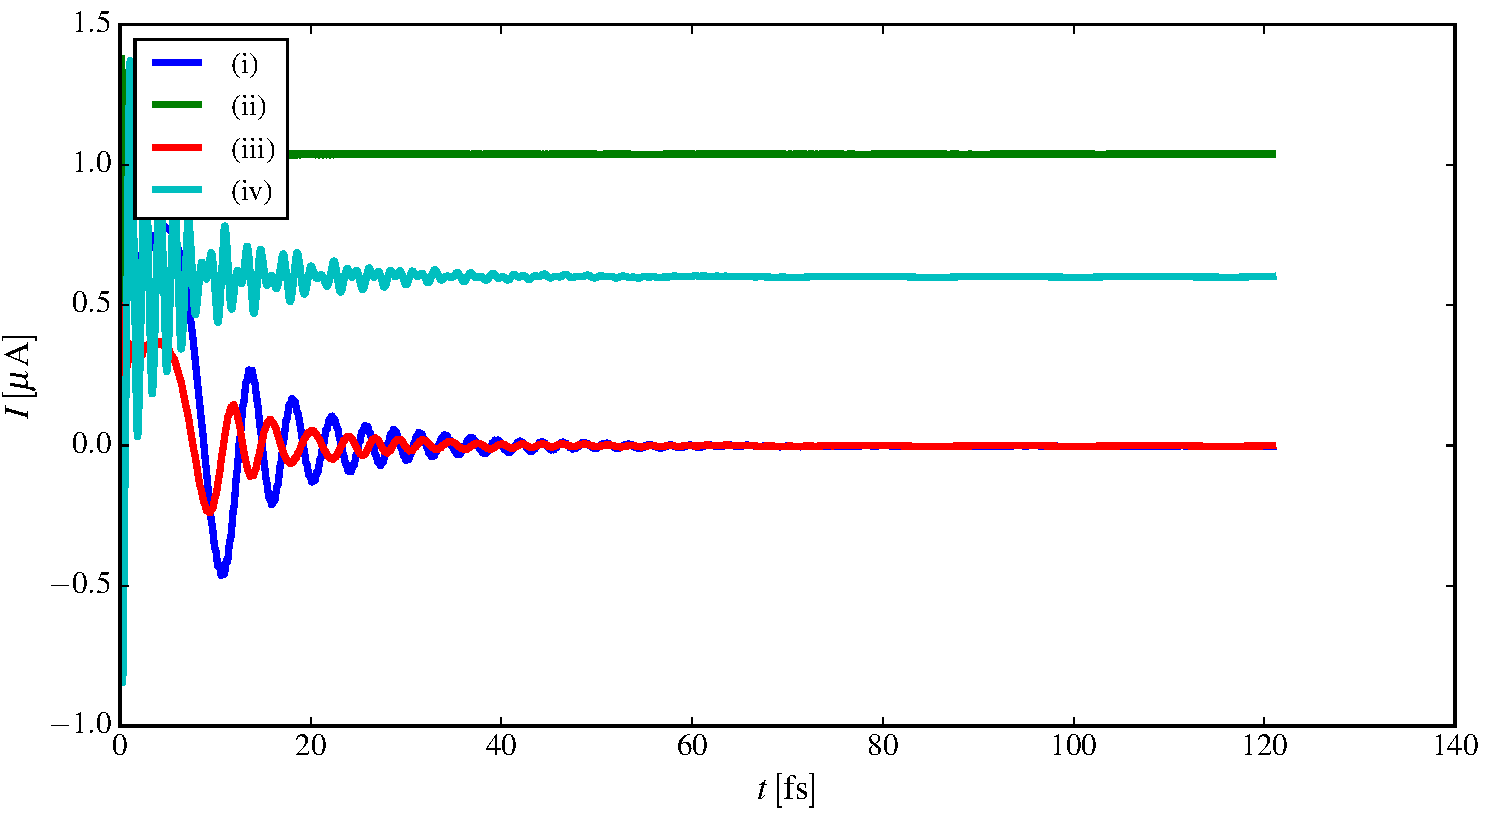
\includegraphics[width=0.9\textwidth]{figs/Peierls_L2_NewParams_Cases_Vvar_currents.pdf}
		\caption{Symmetrized current for the cases discussed above.}\label{fig:Peierls_L2_SimpleParams_Cases_currents}
	\end{figure}
	\begin{figure}[!h]
		\centering
		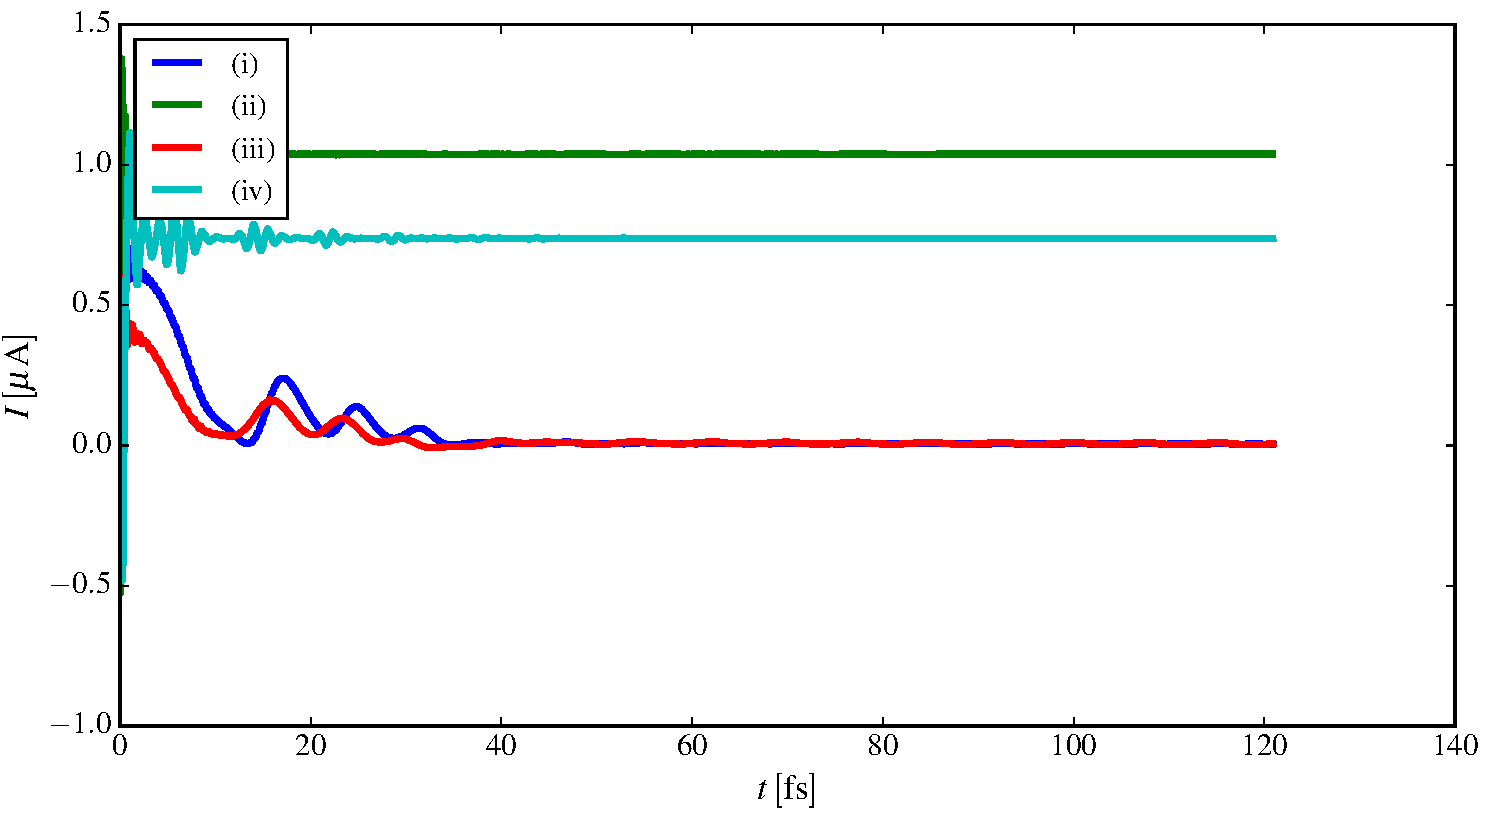
\includegraphics[width=0.9\textwidth]{figs/Peierls_L2_NewParams_Cases_Vvar_currents_avg.pdf}
		\caption{Same as in \cref{fig:Peierls_L2_SimpleParams_Cases_currents}, averaged over 6000 trajectories.}\label{fig:Peierls_L2_SimpleParams_Cases_currents_avg}
	\end{figure}
	\begin{figure}[!h]
		\centering
		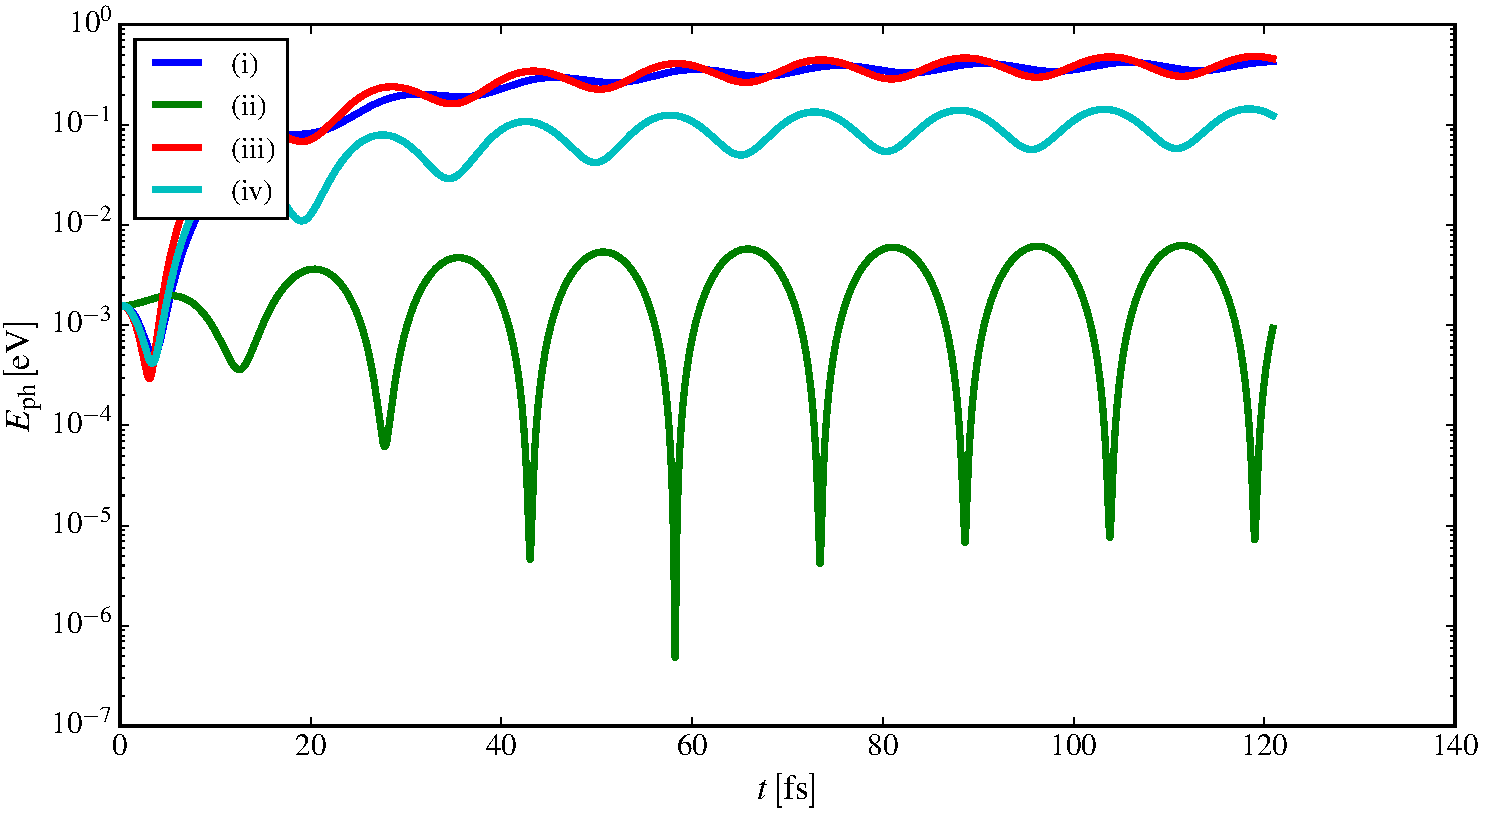
\includegraphics[width=0.9\textwidth]{figs/Peierls_L2_NewParams_Cases_Vvar_phonons.pdf}
		\caption{Vibrational energy for the cases discussed above.}\label{fig:Peierls_L2_SimpleParams_Cases_phonons}
	\end{figure}
	\begin{figure}[!h]
		\centering
		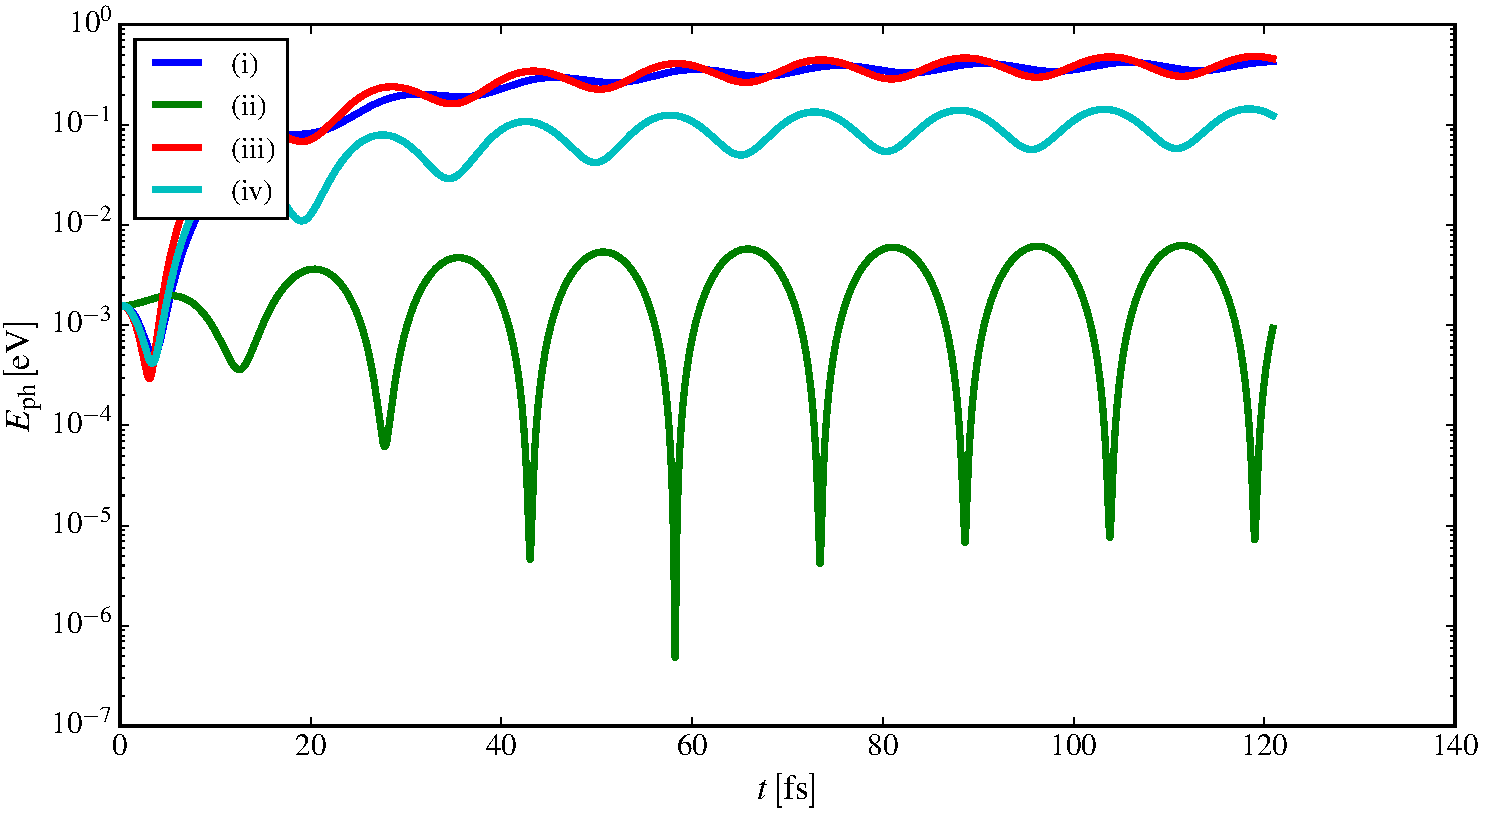
\includegraphics[width=0.9\textwidth]{figs/Peierls_L2_NewParams_Cases_Vvar_phonons.pdf}
		\caption{Same as in \cref{fig:Peierls_L2_SimpleParams_Cases_phonons}, averaged over 6000 trajectories.}\label{fig:Peierls_L2_SimpleParams_Cases_phonons_avg}
	\end{figure}
	\begin{figure}[!h]
		\centering
		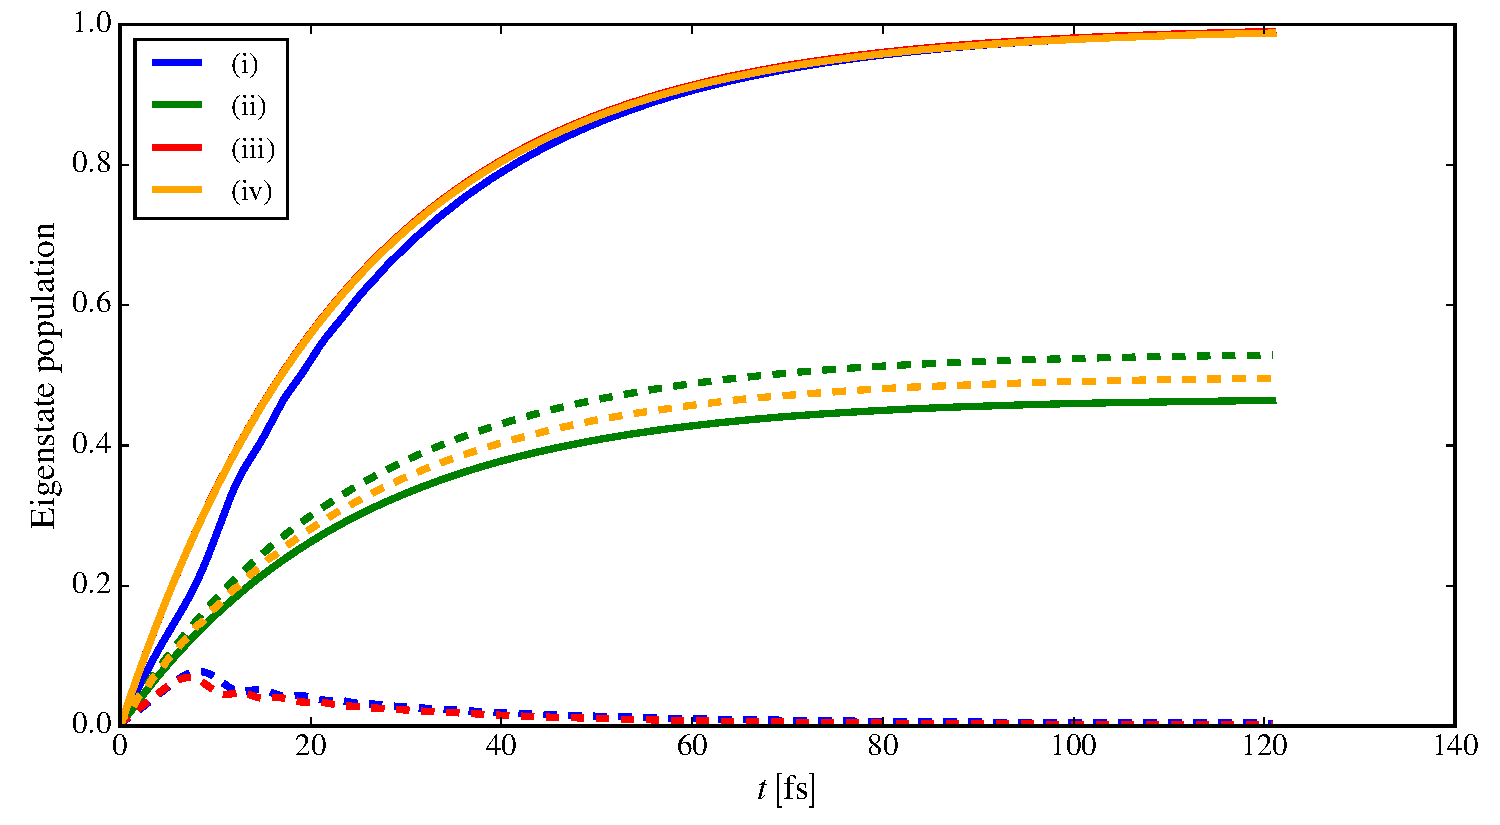
\includegraphics[width=0.9\textwidth]{figs/Peierls_L2_NewParams_Cases_Vvar_ES.pdf}
		\caption{Eigenstate population for the cases discussed above.}\label{fig:Peierls_L2_SimpleParams_Cases_ES}
	\end{figure}
	\begin{figure}[!h]
		\centering
		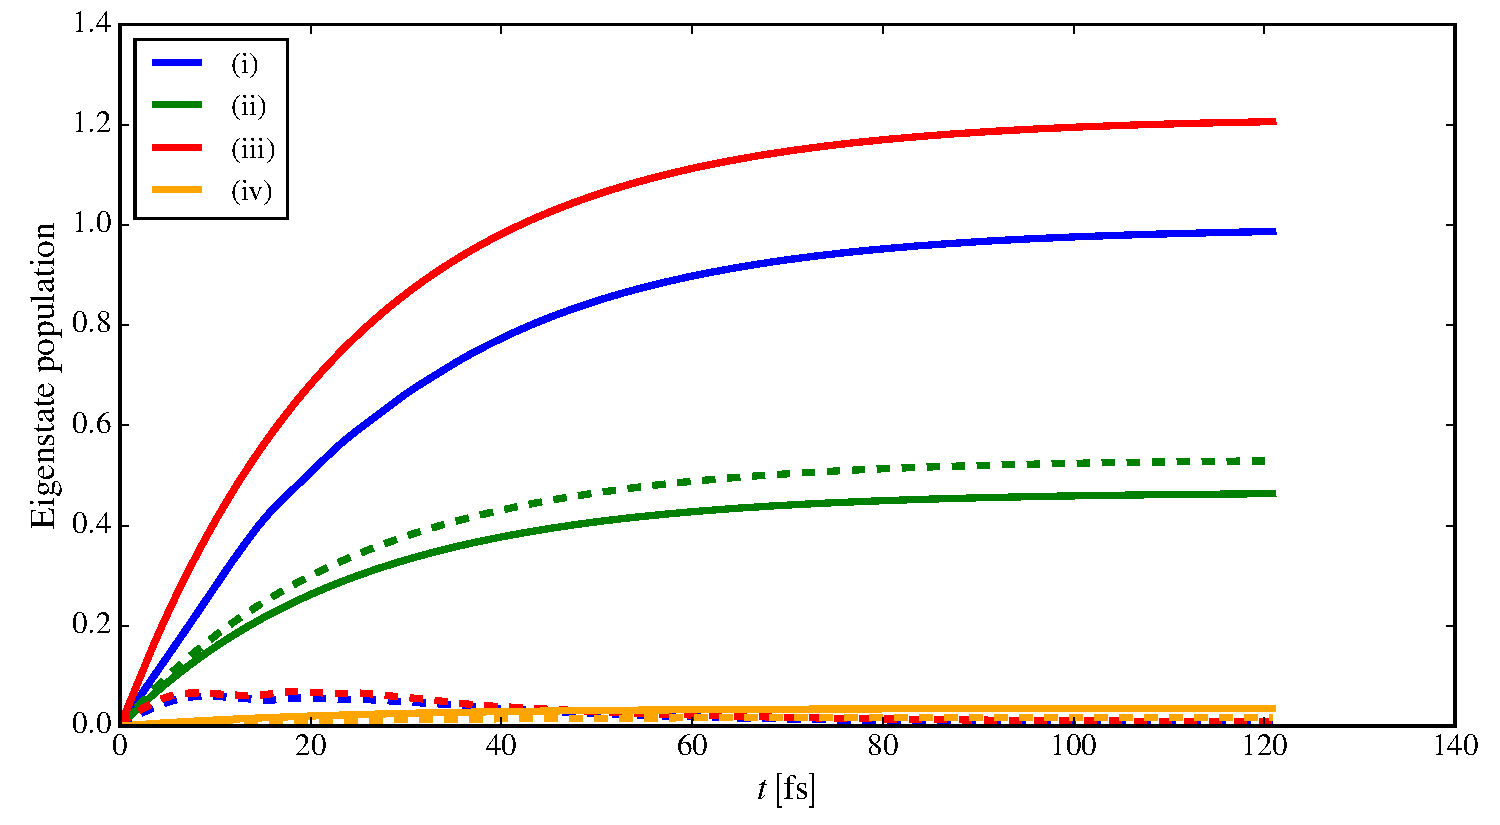
\includegraphics[width=0.9\textwidth]{figs/Peierls_L2_NewParams_Cases_Vvar_ES_avg.pdf}
		\caption{Same as in \cref{fig:Peierls_L2_SimpleParams_Cases_ES}, averaged over 6000 trajectories.}\label{fig:Peierls_L2_SimpleParams_Cases_ES_avg}
	\end{figure}
	\begin{figure}[!h]
		\centering
		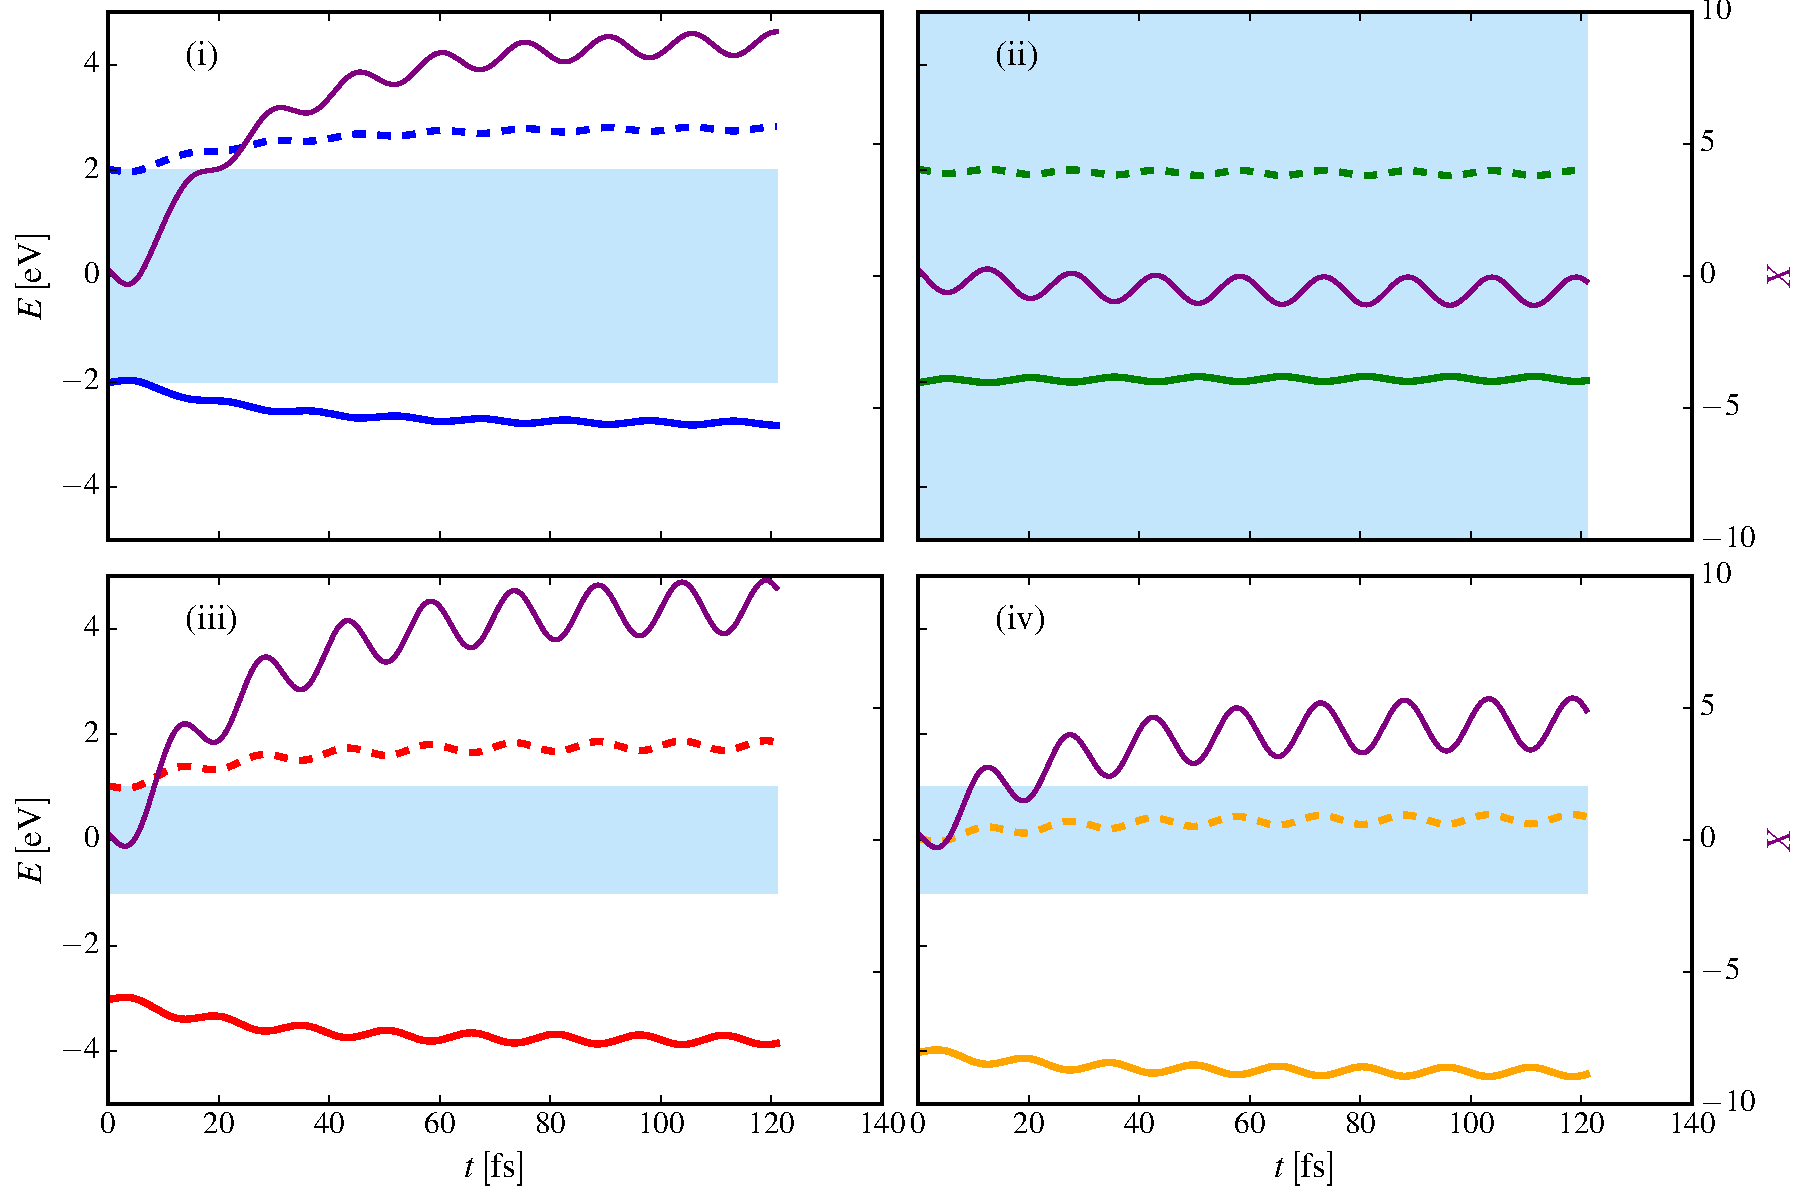
\includegraphics[width=1.0\textwidth]{figs/Peierls_L2_NewParams_Cases_EL_ParVar_Ph.pdf}
		\caption{Eigenlevels and vibrational position (purple) for the cases discussed above.}\label{fig:Peierls_L2_SimpleParams_Cases_El_vib}
	\end{figure}
	\clearpage
	\begin{figure}[!h]
		\centering
		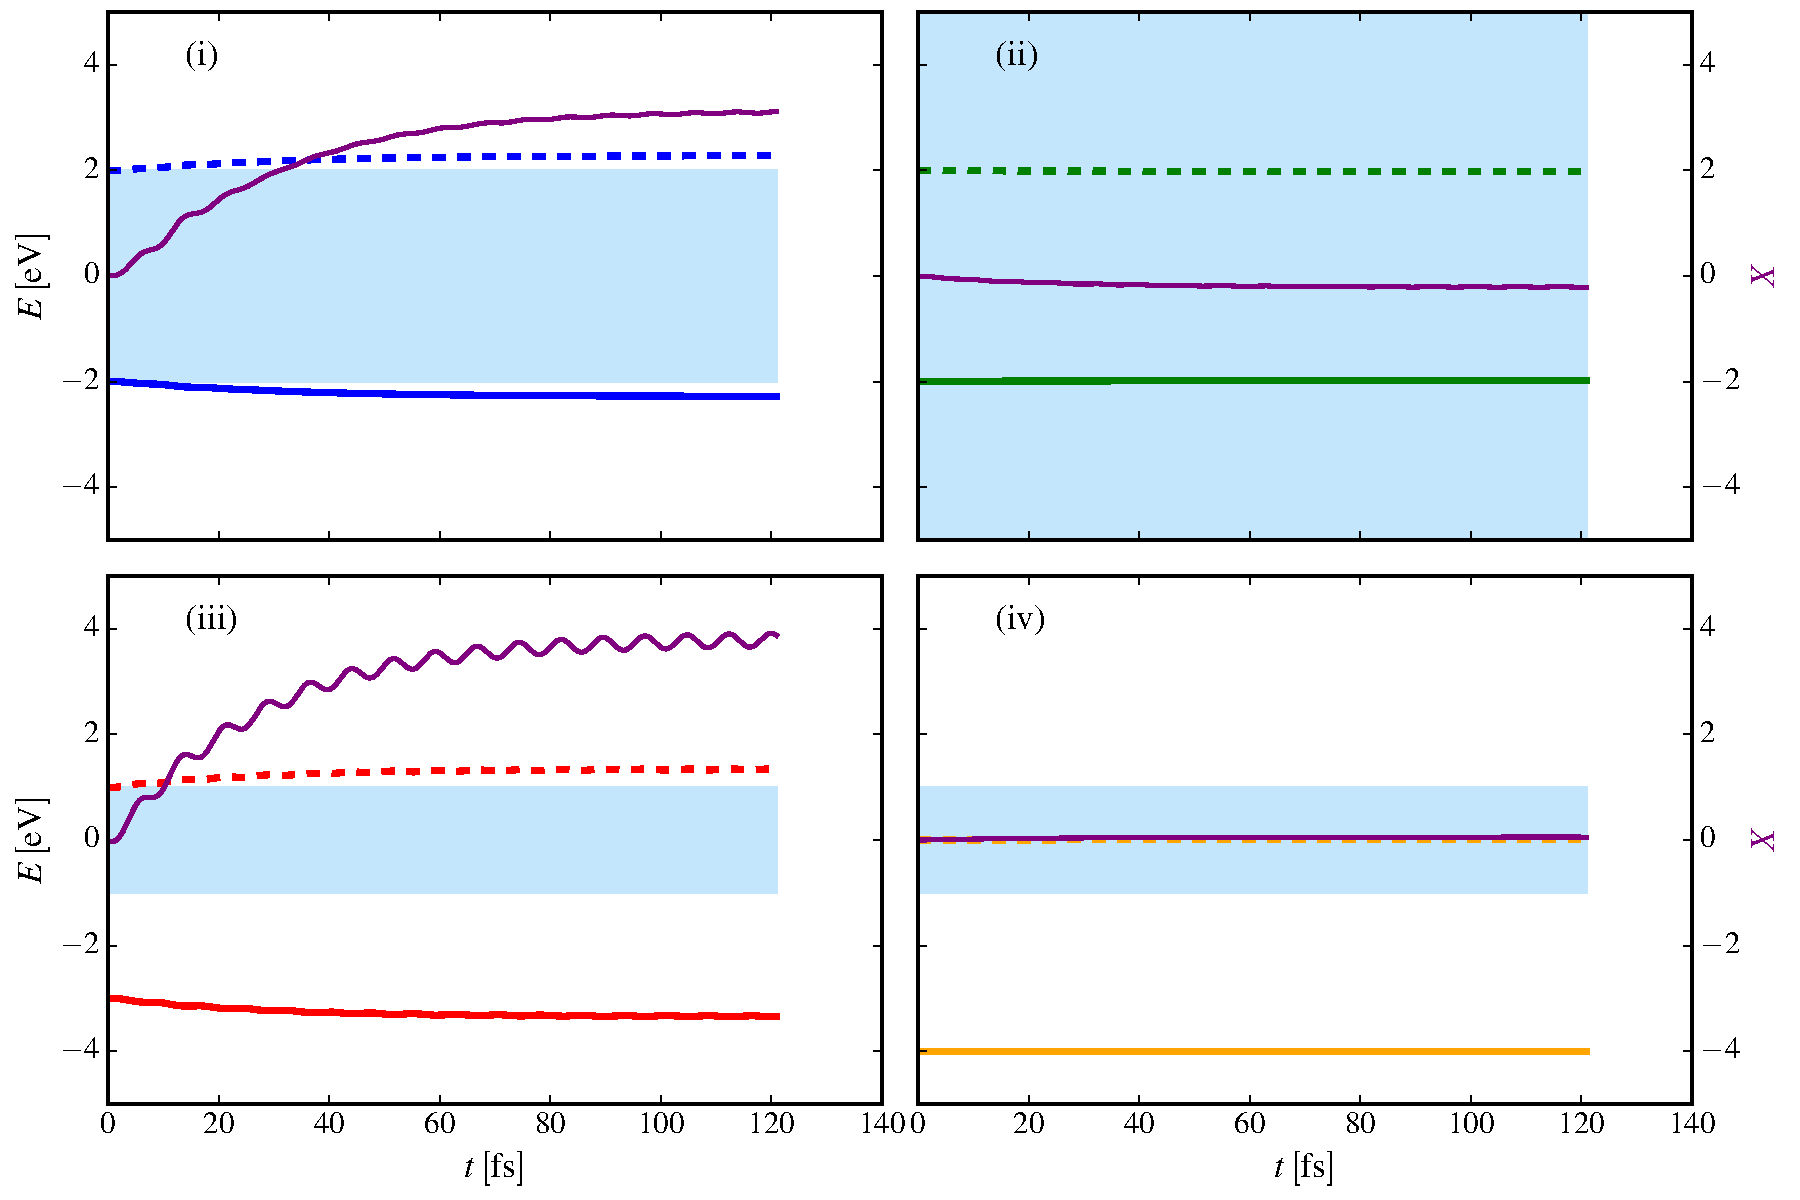
\includegraphics[width=1.0\textwidth]{figs/Peierls_L2_NewParams_Cases_EL_ParVar_Ph_avg.pdf}
		\caption{Same as in \cref{fig:Peierls_L2_SimpleParams_Cases_El_vib}, averaged over 6000 trajectories.}\label{fig:Peierls_L2_SimpleParams_Cases_El_vib_avg}
	\end{figure}
\end{itemize}
\section{Effect of quantum nuclei}
In the previous section, we showed the charge current and vibrational dynamics, and its effects on the electronic spectrum, under a bias voltage in a junction with a classical Peierls model as the central system. Herein, the time-scale of charge dynamics from the leads into the molecule was determined mainly by the $\Gamma$. Treating the vibrational mode classically leads to a change in the electronic spectrum due to the linear dependence of the energy-gap $\Delta \varepsilon$ on the vibrational position $X$ (see \cref{eq:GapXDep}). Since $\omega>\Gamma$, the vibrational mode readjusted to the new vibrational potential $U(X,t)$, which is the harmonic potential modified by a linear term proportional to the instantaneous eigenstate population difference (\cref{eq:VibPotentialMF}), quickly enough and saturated in the minimum of the potential energy (\cref{eq:VibPotentialMF_minimum}). 

One questions is thus, how much does the classical approximation deviate from the full quantum solution. To obtain a first step into this direction, we compute the dynamics of a quantum vibrational mode in the time-dependent mean-field potential given in \cref{eq:VibPotentialMF}, given the numerical solution of the eigenstate population difference $\vert c_-\vert^2 - \vert c_+\vert^2$, by solving the time-dependent Schrödinger equation under the Hamiltonian
\begin{equation}
	H_\mathrm{vib} = \omega a^\dagger a - t_1 (\vert c_-(t)\vert^2 - \vert c_+(t)\vert^2) (a^\dagger + a).
\end{equation} 
This approach assumes that the effect of the vibration on the electrons is the same as in the Ehrenfest approach discussed above. This assumption has to be scrutinized on its own, but will not be investigated further here, but elsewhere.
\subsection{Slow vibrational dynamics}
\Cref{fig:PhQ_vs_PhC_SimpleParams} shows a comparison between such a quantum treatment of the molecular vibration under the mean-field potential arising from the electron-vibrational coupling (black line) with the Ehrenfest-HEOM approach (red line) for various voltage. The parameters used here are the same as in \cref{sec:SimpleParams}. 
\Cref{fig:PhQ_nv_SimpleParams} shows the occupation probability at time $t_\mathrm{f} = \SI{250}{\femto\second}$ of a harmonic oscillator eigenstate with quantum number $n$. 
The eigenstates are of the initial potential, which is 
\begin{equation}
	U(X) = \frac{\omega^2X^2}{2}
\end{equation}
since the molecule is initially unoccupied and the population difference is thus zero.
Generally, the agreement between the quantum dynamics approach and the Ehrenfest-HEOM depends on the used parameters. For example, the position dynamics agrees nearly perfectly for $V= \SI{4.4}{\volt}$, while for $V=\SI{2}{\volt}$ the vibrational mode oscillates around a potential energy minimum, which appears to be shifted by 0.5 in comparison to the one in the Ehrenfest treatment. For high bias voltage $V=\SI{5}{\volt}$, the Ehrenfest approach predicts a much greater oscillation amplitude than the quantum approach. However, these deviations are, compared to the following analysis, relatively small and one can say that for the simplified parameters, treating the vibrational mode classically is a good approximation. 
The population of vibrational eigenstates, shown in \cref{fig:PhQ_nv_SimpleParams}, shows however, that except for high voltage $V=\SI{5}{\volt}$, excited states of the initial harmonic oscillator potential are populated. This makes sense, because for smaller voltages the potential $U(X)$ changes considerably, whereas for $V=\SI{5}{\volt}$ the population difference is nearly zero and thus the potential approximately remains unchanged over time.  
\begin{figure}[!h]
	\centering
	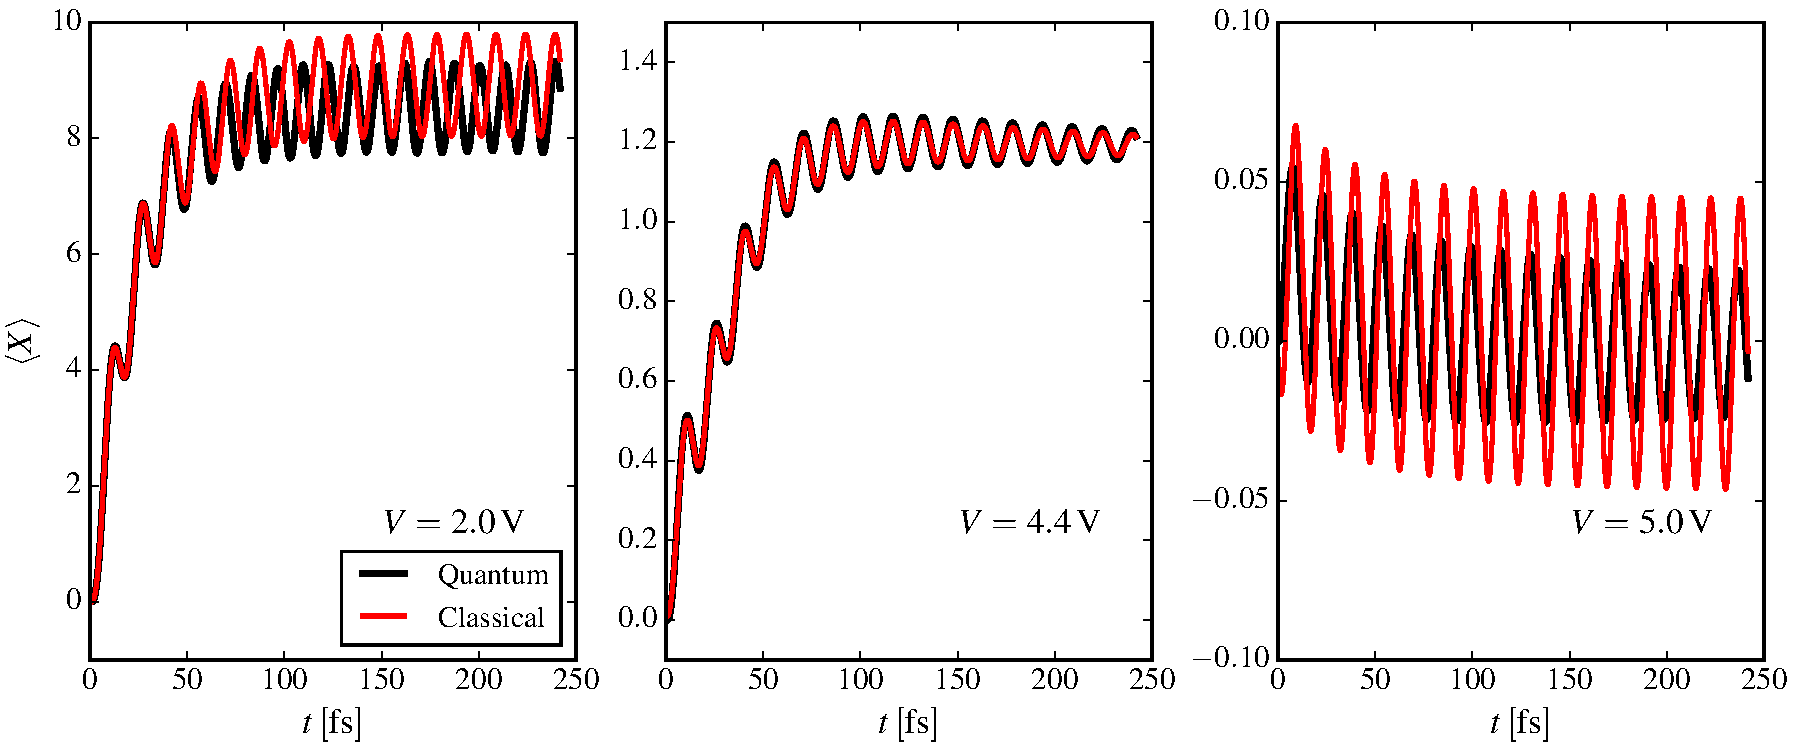
\includegraphics[width=1.0\textwidth]{figs/Peierls_L2_NewParams_PhQ.pdf}
	\caption{Comparison of vibrational postion dynamics for different voltages within a quantum treatment of the vibration with the mean-field potential given in \cref{eq:VibPotentialMF} (black line), and the Ehrenfest-HEOM (red line). The parameters are as in \cref{sec:SimpleParams}.}\label{fig:PhQ_vs_PhC_SimpleParams}
\end{figure} 
\begin{figure}[!h]
	\centering
	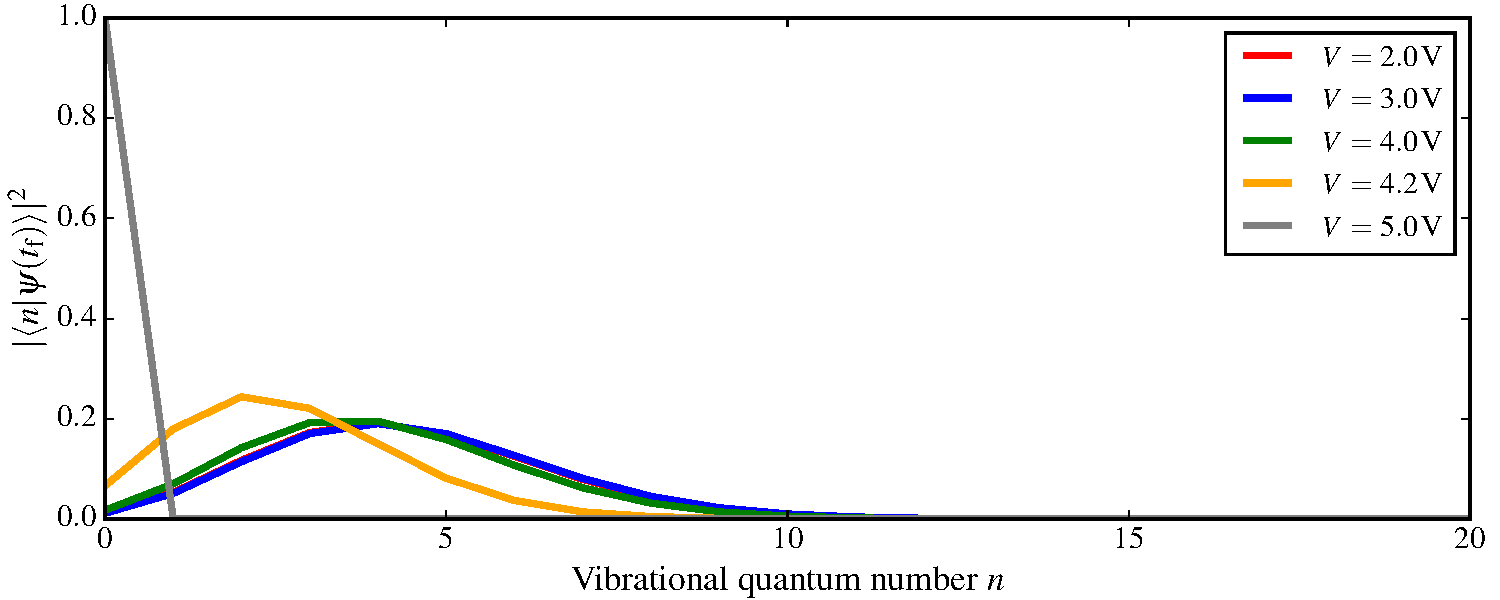
\includegraphics[width=1.0\textwidth]{figs/Peierls_L2_NewParams_PhQ_nv.pdf}
	\caption{Population of vibrational eigenstates for different voltages.}\label{fig:PhQ_nv_SimpleParams}
\end{figure}\\
The time-dependence of the potential can be transferred into the time-dependence of the bosonic ladder operators by the shift-operator $D(\beta)$. Since the minimum of the vibrational potential energy changes as
\begin{equation}
	X_\mathrm{min}(t) = X_\mathrm{min}(t_\mathrm{i}) + \underbrace{t_1\sqrt{\frac{2}{\omega^3}}(\vert c_-(t)\vert^2 - \vert c_+(t)\vert^2)}_{\equiv \alpha(t)},\label{eq:Alpha(t)}
\end{equation}
it is easy to show that this corresponds to 
\begin{equation}
	\tilde{X}(t) = X+\alpha(t) =\sqrt{\frac{1}{2\omega}} (\tilde{a}^\dagger(t) + \tilde{a}(t))
\end{equation}
with
\begin{equation}
	\tilde{a}(t) = D^\dagger (\beta(t)) aD (\beta(t))
\end{equation}
and the displacement operator is defined as 
\begin{equation}
	D(\beta) = \exp\left(\beta a^\dagger - \beta^* a\right).
\end{equation}
In our case, the shift-parameter $\beta$ is given by the displacement of the vibrational energy $\alpha(t)$ at time $t$
\begin{equation}
	\beta(t) = \sqrt{\frac{\omega}{2}} \alpha(t).
\end{equation}
The population of vibrational states of the shifted potential is shown in \cref{fig:PhQ_nv_SimpleParams_shifted}. It shows that the vibrational wavefunction remains in the ground state of the instantaneous mean-field potential $U(X,t)$ throughout the full time-evolution. In this regard, for the parameters investigated here, quantum vibrational dynamics is adiabatic in the mean-field time-dependent potential produced by the electrons.
\begin{figure}[!h]
	\centering
	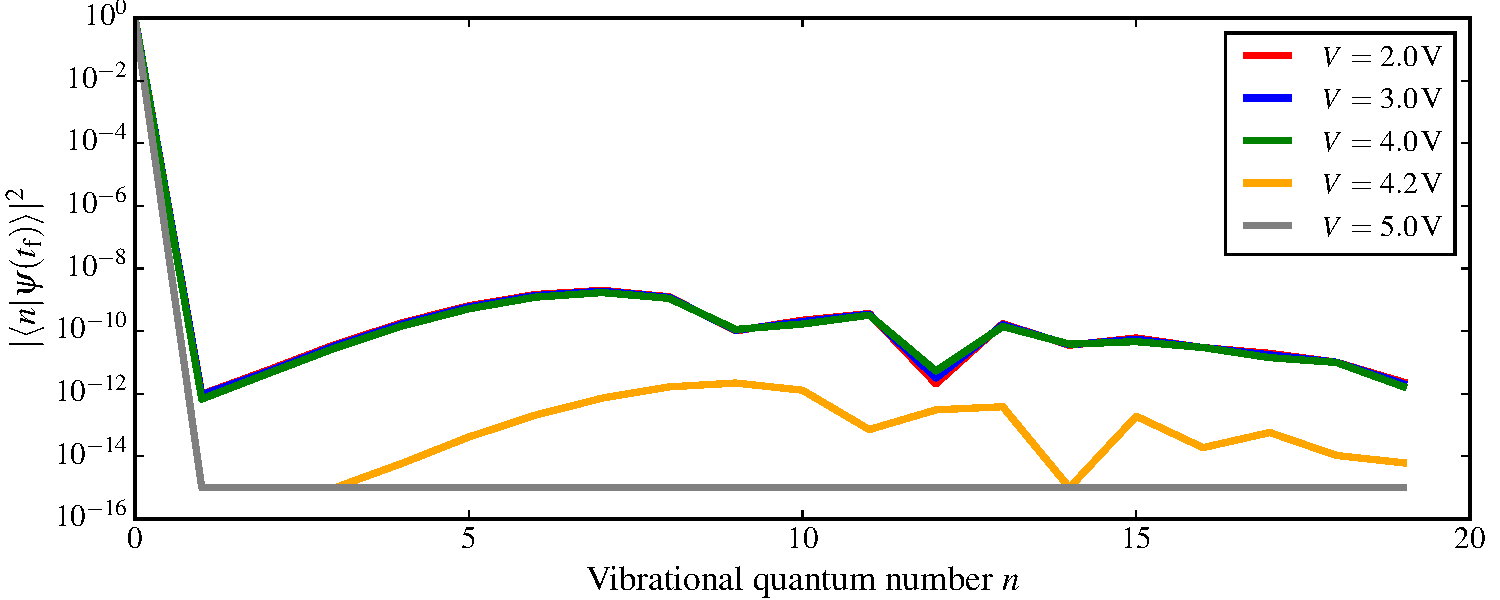
\includegraphics[width=1.0\textwidth]{figs/Peierls_L2_NewParams_PhQ_nv_shifted.pdf}
	\caption{Population of vibrational eigenstates for different voltages in the harmonic oscillator eigenbasis shifted by $\alpha(t)$ as defined in \cref{eq:Alpha(t)}.}\label{fig:PhQ_nv_SimpleParams_shifted}
\end{figure} 
\clearpage
\subsection{Parameters used by Fransson}
We now turn to the comparison between a quantum treatment of the vibrational mode and the Ehrenfest approach for the parameters of the original problem. Again, \cref{fig:PhQ_vs_PhC_FranssonParams} shows a comparison of the quantum treatment and the Ehrenfest-HEOM for selected voltages. 
The voltages are chosen for representative situations, schematically shown in \cref{fig:Schematic_Voltages_FranssonParams}. $V=\SI{0}{\volt}$ corresponds to both levels below Fermi-level, $V=\SI{0.4}{\volt}$ to the right lead chemical potential resonant with $\varepsilon_+$, $V=\SI{0.48}{\volt}$ to $\mu_R$ in the middle between $\varepsilon_+$ and $\varepsilon_-$, $V=\SI{0.56}{\volt}$ to the case where the upper level is in the bias window and $\mu_R=\varepsilon_-$, and finally $V=\SI{0.8}{\volt}$ to the high-bias regime in which both levels are in the bias window.
Similarly to the parameters investigated above, the Ehrenfest-approach agrees with the quantum treatment particularly well when both levels are inside the bias window but the voltage is not too large. In the low bias regime and for very large voltages, the oscillation amplitudes and frequencies, and also the damping is different in both approaches. 
\Cref{fig:PhQ_nv_FranssonParams} shows the nuclear wave functions (at time $t_\mathrm{f} = \SI{12}{\pico\second}$) occupation number probability. Contrary to the previous parameters, the vibrational wavefunction remains mostly in the ground state for $V=\SI{0}{\volt}$ (all levels fully occupied since they are below Fermi-level) and $V=\SI{0.8}{\volt}$ (all levels in the bias window). For intermediate voltages $V=\SI{0.4}{\volt}$ and $V=\SI{0.56}{\volt}$, the highest lying state with a finite occupation probability is $n=3$. Thus, the wave-function can be described by the ground state and the first, second and third vibrational excited state. 
\begin{figure}[!h]
	\centering
	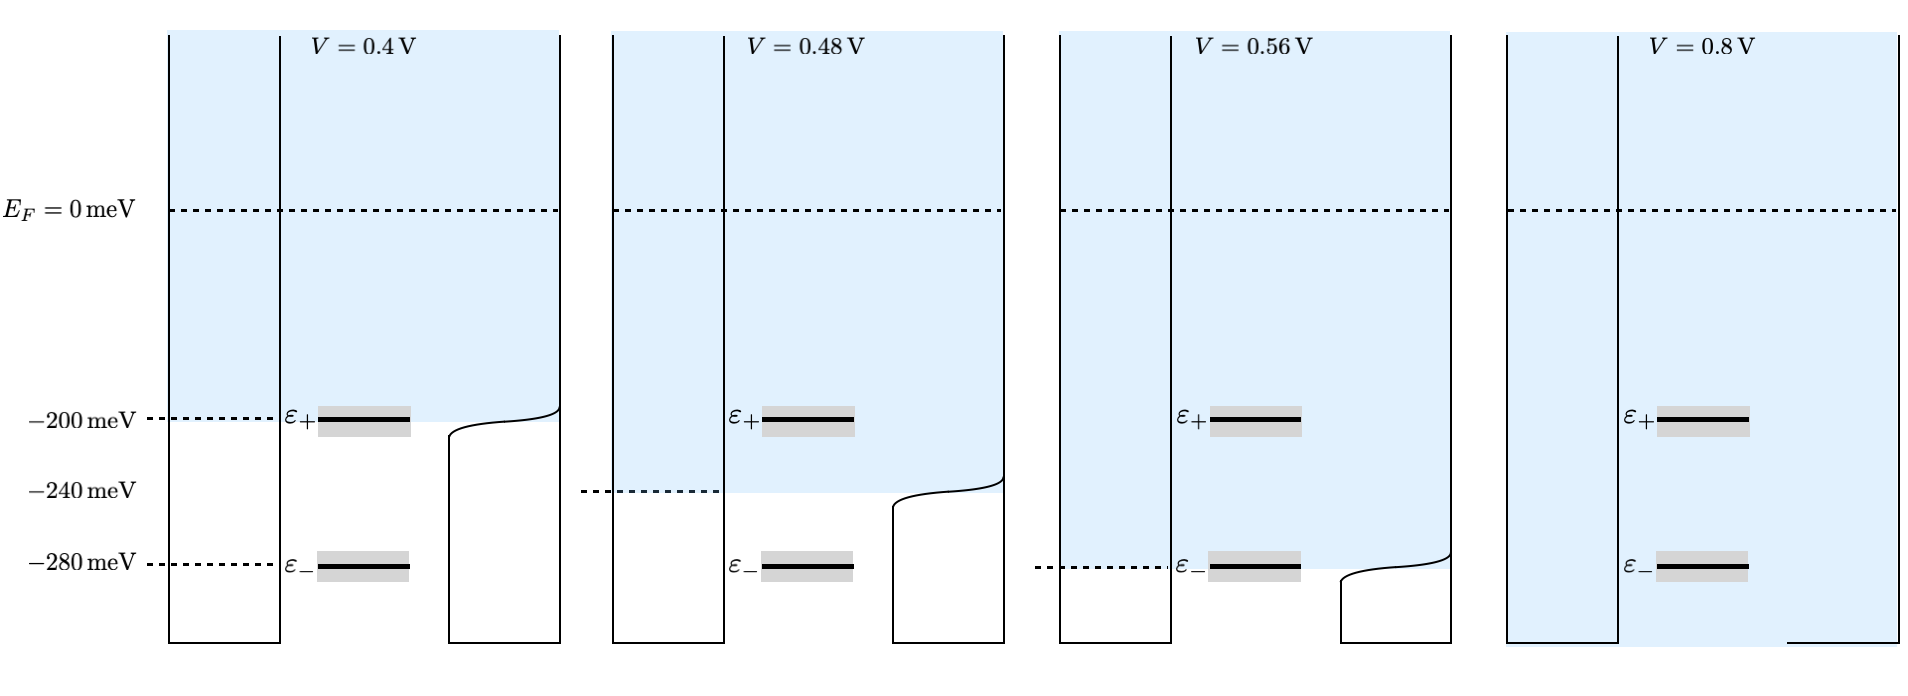
\includegraphics[width=1.0\textwidth]{figs/Schematic_Voltages_FranssonParams.png}
	\caption{Schematic of the investigated voltage regimes of the spinless two-site Peierls model with the original Parameters.}\label{fig:Schematic_Voltages_FranssonParams}
\end{figure}
\begin{figure}[!h]
	\centering
	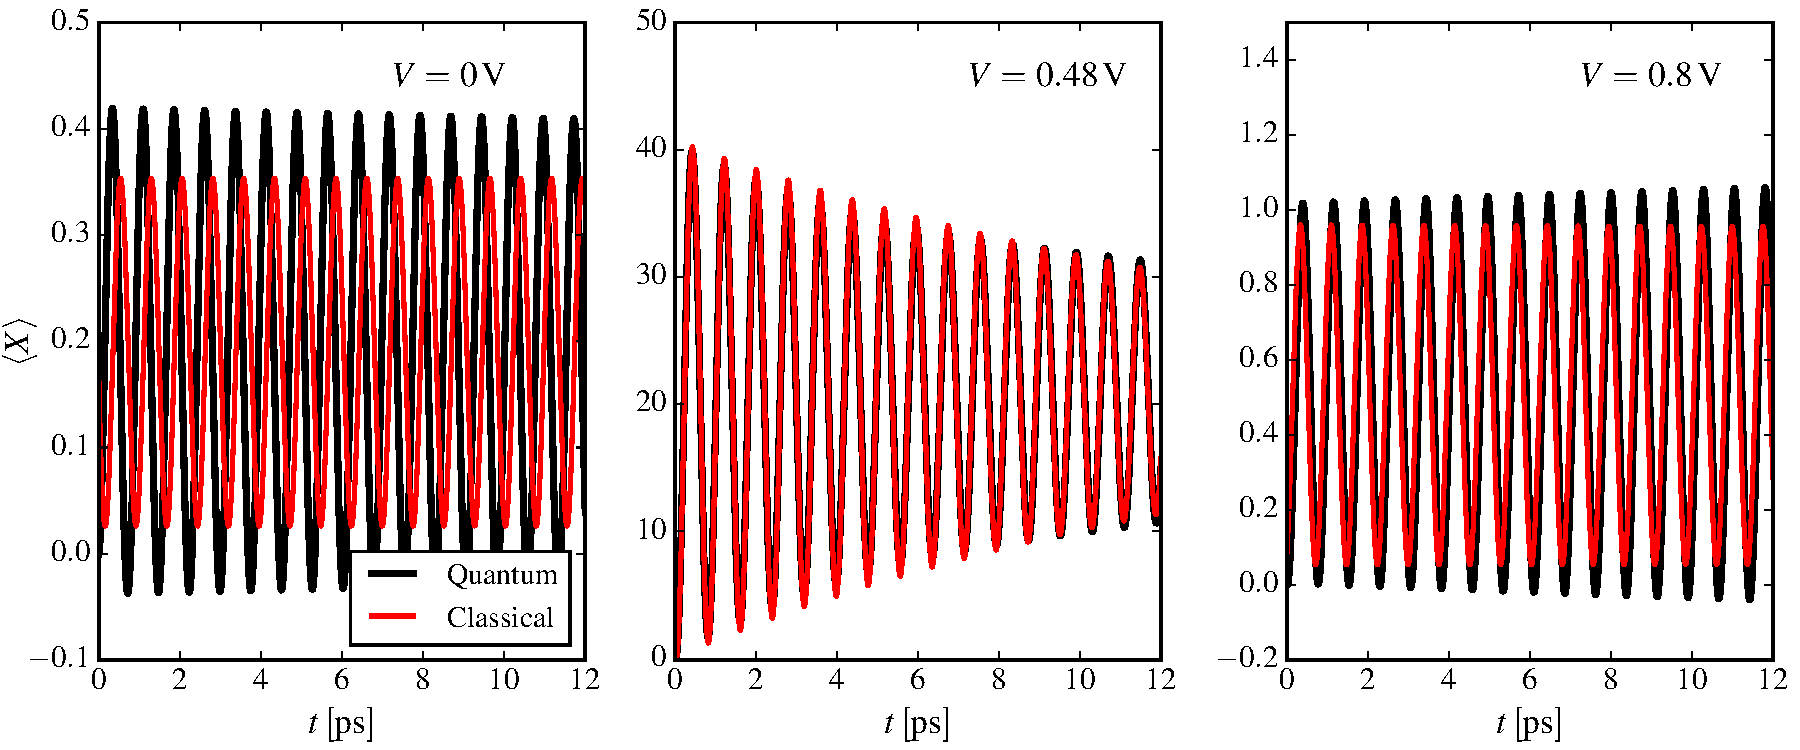
\includegraphics[width=1.0\textwidth]{figs/Peierls_L2_FranssonParams_PhQ.pdf}
	\caption{Comparison of vibrational postion dynamics for different voltages within a quantum treatment of the vibration with the mean-field potential given in \cref{eq:VibPotentialMF} (black line), and the Ehrenfest-HEOM (red line). The parameters are as in \cref{sec:Aim}.}\label{fig:PhQ_vs_PhC_FranssonParams}
\end{figure} 
\clearpage
\begin{figure}[!h]
	\centering
	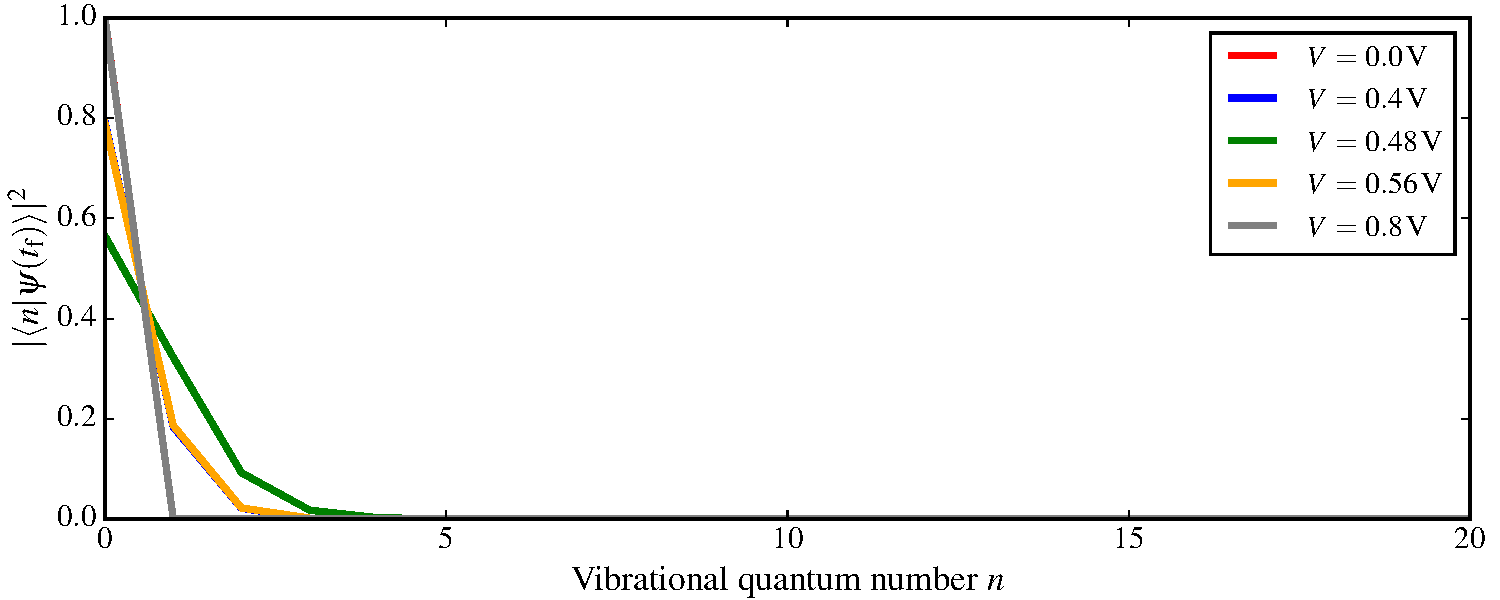
\includegraphics[width=1.0\textwidth]{figs/Peierls_L2_FranssonParams_PhQ_nv.pdf}
	\caption{Population of vibrational eigenstates for different voltages for the original parameters.}\label{fig:PhQ_nv_FranssonParams}
\end{figure} 
\section{Effect of classical nuclei within the full HEOM}
The previous analysis suggests that both for the simplified and the original parameters, treating the vibrational mode classically is agreeing well with an approach, in which the vibrational mode is treated quantum-mechanically but it is in a mean-field potential produced by the population difference. Underlying the latter approach is the assumption, that charge dynamics is determined by states in the single-excitation subspace only. The aim of this section is to investigate the validity of the single-particle approximation. 
Since $\Gamma$ is smaller than all other parameters, my expectation is that sequential tunneling, which should be captured by the single-particle approximation, is the dominant process, whereas co-tunneling and higher order processes are unlikely (this might be rubbish).  
\section{Comparison of Ehrenfest with full HEOM}
In this section we investigate the Peierls model without the above mentioned approximations within the full HEOM. 
\subsection{Fransson parameters}
Here, we use the parameters used by Fransson, as given in \cref{sec:Aim}.
\subsection{Parameter set 1}
%\section{Born-Oppenheimer potential energy analysis }
\section{Ground State of the two-site Peierls model}
\subsection{Classical vibration}
The Peierls-Hamiltonian within the classical vibration approximation can be diagonalized exactly.
Herein, the basis states are $\vert n_1 n_2\rangle$ with $n_1,n_2=0,1$. In this basis, the Hamiltonian reads
\begin{equation}
	H = \begin{pmatrix}
		0 & 0 & 0 & 0\\
		0 & \varepsilon & -t_0-\sqrt{2\omega}t_1X & 0\\
		0 & -t_0-\sqrt{2\omega}t_1X & \varepsilon & 0\\
		0 & 0 & 0 & 2\varepsilon
	\end{pmatrix}
\end{equation}
where we used the ordering $\vert 00\rangle,\vert 01\rangle,\vert 10\rangle,\vert 11\rangle$. The corresponding eigenvalues and eigenstates are
\begin{align}
	\varepsilon_e &= 0\qquad & \vert \psi_e\rangle &= \vert 00\rangle\\
	\varepsilon_o &= 2\varepsilon\qquad & \vert \psi_o\rangle &= \vert 11\rangle\\
	\varepsilon_\pm &= \varepsilon\pm \vert t_0+t_1\sqrt{2\omega}X\vert \qquad &\vert \psi_\pm\rangle &= \frac{1}{\sqrt{2}}(\vert 01\rangle \pm \vert 10\rangle).
\end{align}
For the simplified parameter considered above, the empty ($\vert\psi_u\rangle$) and doubly occupied ($\vert \psi_o\rangle$) molecular states are degenerate. The remaining two states, the bonding and anti-bonding states, are the same as in the single-particle formulation applied in the previous sections. The ground state is for $t_0=\SI{2}{\electronvolt}$, $\omega=\SI{0.1}{\electronvolt}$ and $t_1=\SI{0.2}{\volt}$ is the anti-bonding state $\vert\psi_-\rangle$.
\subsection{Influence of on-site potential}
In the limit of $\varepsilon\rightarrow-\infty$ the ground state of the Fransson model is a product state of doubly occupied electronic sites and all vibrational modes in their lowest energy state
\begin{equation}
	\vert \Psi_\mathrm{GS}\rangle = \vert \uparrow\downarrow,\uparrow\downarrow,\dots,\uparrow\downarrow\rangle\vert 0,\dots,0\rangle.
\end{equation}
\subsection{Influence of Hopping}
Hopping tends to delocalize electrons and due to its off-diagonal contribution the ground state is a superposition over many configurations. The dominant one is with half filling with one electron per site. Contributions with smaller weight are ones in which a single site is doubly occupied and one is empty, while all others are singly occupied. The table below shows representative configurations for $t_0 = \SI{40}{\electronvolt}$ and $\varepsilon = \SI{0}{\electronvolt}$ for $L=6$ (due to spin-flip and translational symmetry of the model in this limit, many configurations are degenerate).
\begin{center}
\begin{tabular}{cc}
	Configuration & Weight\\
	\hline
	$\vert \uparrow,\downarrow,\uparrow,\downarrow,\uparrow,\downarrow\rangle $&  0.1250\\
	$\vert \downarrow,\uparrow\downarrow,0,\uparrow,\downarrow,\uparrow\rangle $&  0.0833\\
	$\vert \uparrow\downarrow,0,\uparrow,\uparrow\downarrow,\downarrow,0\rangle $&  0.0555\\
	$\vert \uparrow,\downarrow,\uparrow\downarrow,\downarrow,\uparrow,0\rangle $&  0.0416\\
	$\vert \uparrow\downarrow,0,\uparrow,\uparrow,\downarrow,\downarrow\rangle $&  0.0277\\
	$\vert \uparrow\downarrow,0,\uparrow\downarrow,0,\uparrow\downarrow,0\rangle$&  -0.1250\\
	\hline
\end{tabular}
\end{center}
\subsection{Influence of Peierls-coupling}
\section{Nonadiabatic transition matrix elements}
\subsection{Spinless Peierls model}
Aka two-level one-mode model with nonadiabatic coupling. 
\end{document}




